% Options for packages loaded elsewhere
\PassOptionsToPackage{unicode}{hyperref}
\PassOptionsToPackage{hyphens}{url}
%
\documentclass[
  14pt,
  ignorenonframetext,
  aspectratio=169,
]{beamer}
\usepackage{pgfpages}
\setbeamertemplate{caption}[numbered]
\setbeamertemplate{caption label separator}{: }
\setbeamercolor{caption name}{fg=normal text.fg}
\beamertemplatenavigationsymbolsempty
% Prevent slide breaks in the middle of a paragraph
\widowpenalties 1 10000
\raggedbottom

\usepackage{amsmath,amssymb}
\usepackage{iftex}
\ifPDFTeX
  \usepackage[T1]{fontenc}
  \usepackage[utf8]{inputenc}
  \usepackage{textcomp} % provide euro and other symbols
\else % if luatex or xetex
  \usepackage{unicode-math}
  \defaultfontfeatures{Scale=MatchLowercase}
  \defaultfontfeatures[\rmfamily]{Ligatures=TeX,Scale=1}
\fi
\usepackage{lmodern}
\usetheme[]{monash}
\ifPDFTeX\else  
    % xetex/luatex font selection
\fi
% Use upquote if available, for straight quotes in verbatim environments
\IfFileExists{upquote.sty}{\usepackage{upquote}}{}
\IfFileExists{microtype.sty}{% use microtype if available
  \usepackage[]{microtype}
  \UseMicrotypeSet[protrusion]{basicmath} % disable protrusion for tt fonts
}{}
\makeatletter
\@ifundefined{KOMAClassName}{% if non-KOMA class
  \IfFileExists{parskip.sty}{%
    \usepackage{parskip}
  }{% else
    \setlength{\parindent}{0pt}
    \setlength{\parskip}{6pt plus 2pt minus 1pt}}
}{% if KOMA class
  \KOMAoptions{parskip=half}}
\makeatother
\usepackage{xcolor}
\newif\ifbibliography
\setlength{\emergencystretch}{3em} % prevent overfull lines
\setcounter{secnumdepth}{-\maxdimen} % remove section numbering

\usepackage{color}
\usepackage{fancyvrb}
\newcommand{\VerbBar}{|}
\newcommand{\VERB}{\Verb[commandchars=\\\{\}]}
\DefineVerbatimEnvironment{Highlighting}{Verbatim}{commandchars=\\\{\}}
% Add ',fontsize=\small' for more characters per line
\usepackage{framed}
\definecolor{shadecolor}{RGB}{248,248,248}
\newenvironment{Shaded}{\begin{snugshade}}{\end{snugshade}}
\newcommand{\AlertTok}[1]{\textcolor[rgb]{0.94,0.16,0.16}{#1}}
\newcommand{\AnnotationTok}[1]{\textcolor[rgb]{0.56,0.35,0.01}{\textbf{\textit{#1}}}}
\newcommand{\AttributeTok}[1]{\textcolor[rgb]{0.77,0.63,0.00}{#1}}
\newcommand{\BaseNTok}[1]{\textcolor[rgb]{0.00,0.00,0.81}{#1}}
\newcommand{\BuiltInTok}[1]{\textcolor[rgb]{0.00,0.00,0.00}{#1}}
\newcommand{\CharTok}[1]{\textcolor[rgb]{0.31,0.60,0.02}{#1}}
\newcommand{\CommentTok}[1]{\textcolor[rgb]{0.56,0.35,0.01}{\textit{#1}}}
\newcommand{\CommentVarTok}[1]{\textcolor[rgb]{0.56,0.35,0.01}{\textbf{\textit{#1}}}}
\newcommand{\ConstantTok}[1]{\textcolor[rgb]{0.00,0.00,0.00}{#1}}
\newcommand{\ControlFlowTok}[1]{\textcolor[rgb]{0.13,0.29,0.53}{\textbf{#1}}}
\newcommand{\DataTypeTok}[1]{\textcolor[rgb]{0.13,0.29,0.53}{#1}}
\newcommand{\DecValTok}[1]{\textcolor[rgb]{0.00,0.00,0.81}{#1}}
\newcommand{\DocumentationTok}[1]{\textcolor[rgb]{0.56,0.35,0.01}{\textbf{\textit{#1}}}}
\newcommand{\ErrorTok}[1]{\textcolor[rgb]{0.64,0.00,0.00}{\textbf{#1}}}
\newcommand{\ExtensionTok}[1]{\textcolor[rgb]{0.00,0.00,0.00}{#1}}
\newcommand{\FloatTok}[1]{\textcolor[rgb]{0.00,0.00,0.81}{#1}}
\newcommand{\FunctionTok}[1]{\textcolor[rgb]{0.00,0.00,0.00}{#1}}
\newcommand{\ImportTok}[1]{\textcolor[rgb]{0.00,0.00,0.00}{#1}}
\newcommand{\InformationTok}[1]{\textcolor[rgb]{0.56,0.35,0.01}{\textbf{\textit{#1}}}}
\newcommand{\KeywordTok}[1]{\textcolor[rgb]{0.13,0.29,0.53}{\textbf{#1}}}
\newcommand{\NormalTok}[1]{\textcolor[rgb]{0.00,0.00,0.00}{#1}}
\newcommand{\OperatorTok}[1]{\textcolor[rgb]{0.81,0.36,0.00}{\textbf{#1}}}
\newcommand{\OtherTok}[1]{\textcolor[rgb]{0.56,0.35,0.01}{#1}}
\newcommand{\PreprocessorTok}[1]{\textcolor[rgb]{0.56,0.35,0.01}{\textit{#1}}}
\newcommand{\RegionMarkerTok}[1]{\textcolor[rgb]{0.00,0.00,0.00}{#1}}
\newcommand{\SpecialCharTok}[1]{\textcolor[rgb]{0.00,0.00,0.00}{#1}}
\newcommand{\SpecialStringTok}[1]{\textcolor[rgb]{0.31,0.60,0.02}{#1}}
\newcommand{\StringTok}[1]{\textcolor[rgb]{0.31,0.60,0.02}{#1}}
\newcommand{\VariableTok}[1]{\textcolor[rgb]{0.00,0.00,0.00}{#1}}
\newcommand{\VerbatimStringTok}[1]{\textcolor[rgb]{0.31,0.60,0.02}{#1}}
\newcommand{\WarningTok}[1]{\textcolor[rgb]{0.56,0.35,0.01}{\textbf{\textit{#1}}}}

\providecommand{\tightlist}{%
  \setlength{\itemsep}{0pt}\setlength{\parskip}{0pt}}\usepackage{longtable,booktabs,array}
\usepackage{calc} % for calculating minipage widths
\usepackage{caption}
% Make caption package work with longtable
\makeatletter
\def\fnum@table{\tablename~\thetable}
\makeatother
\usepackage{graphicx}
\makeatletter
\def\maxwidth{\ifdim\Gin@nat@width>\linewidth\linewidth\else\Gin@nat@width\fi}
\def\maxheight{\ifdim\Gin@nat@height>\textheight\textheight\else\Gin@nat@height\fi}
\makeatother
% Scale images if necessary, so that they will not overflow the page
% margins by default, and it is still possible to overwrite the defaults
% using explicit options in \includegraphics[width, height, ...]{}
\setkeys{Gin}{width=\maxwidth,height=\maxheight,keepaspectratio}
% Set default figure placement to htbp
\makeatletter
\def\fps@figure{htbp}
\makeatother

% Colors
\definecolor{shadecolor}{RGB}{225,225,225}
\setbeamercolor{description item}{fg=Orange}
\definecolor{MonashBlue}{RGB}{66,109,152}
\definecolor{burntorange}{rgb}{0.8, 0.33, 0.0}

% Packages
\usepackage{amsmath, bm, amssymb, amsthm, mathrsfs,pifont}
\usepackage{url}
\usepackage{multirow, booktabs, float, textcmds, siunitx}
\usepackage{bm,booktabs,animate,ragged2e,multicol,microtype,hyperref}
\usepackage{fontawesome5}

% Figures
\graphicspath{{figs/}}

% Fonts
\fontsize{13}{15}\sf
\setbeamerfont{title}{series=\bfseries,parent=structure,size=\fontsize{24}{24}}
\ifcsname Shaded\endcsname
  \definecolor{shadecolor}{RGB}{225,225,225}
  \renewenvironment{Shaded}{\vspace*{0.15cm}\color{black}\fontsize{10}{10}\sf\begin{snugshade}\color{black}}{\end{snugshade}}
\fi

% gt dependencies
\usepackage{longtable,caption,setspace}
\captionsetup{font={small,stretch=0.80}}

% My definitions

\def\E{\text{E}}
\def\V{\text{Var}}
\def\up#1{\raisebox{-0.3cm}{#1}}
\def\pred#1#2#3{\hat{#1}_{#2|#3}}
\def\damped{$_\text{d}$}
\def\h+{h_{m}^{+}}
\def\str#1{\rlap{#1}\textcolor{red}{\rule{1cm}{0.1cm}}}

\def\st#1{\rlap{#1}\textcolor{red}{\rule{1cm}{0.1cm}}}
\def\bY{\bm{y}}
\def\by{\bm{y}}
\def\bS{\bm{S}}
\def\bI{\text{\rm\textbf{I}}}
\def\bbeta{\bm{\beta}}
\def\bSigma{\bm{\Sigma}}
\def\bW{\bm{\Sigma}}
\def\Var{\text{Var}}
\def\var{\text{Var}}
\def\bOmega{\bm{\Omega}}
\def\bLambda{\bm{\Lambda}}
\let\mc\multicolumn
\def\hl{\color[RGB]{230, 172, 0}}

\def\forecast{\begin{alertblock}{}\fontsize{10}{11}\sf
 A forecast is an estimate of the probability distribution of a variable to be observed in the future.
\end{alertblock}}

\def\simfutures{\begin{textblock}{2.9}(12.8,7.7)
\begin{block}{}\fontsize{10}{11}\sf
Simulated futures from an ETS model
\end{block}\end{textblock}}

\setbeamertemplate{title page}
{\placefig{0}{-0.5}{width=1.01\paperwidth,height=1.45\paperheight}{africa1.jpg}
\begin{textblock}{8.5}(.5,0.2)
  \raggedright\fontsize{20}{20}\selectfont\bfseries\sffamily\textcolor{white}{\inserttitle}\\[0.2cm]
  \fontsize{12}{12}\selectfont\bfseries\sffamily\textcolor{white}{\insertsubtitle}
  \end{textblock}
\placefig{.5}{6.2}{width=2.4cm}{tsibble.png}
\placefig{2.9}{6.2}{width=2.4cm}{feasts.png}
\placefig{5.3}{6.2}{width=2.4cm}{fable.png}
\begin{textblock}{7.5}(10.6,-.1)
  {\fontsize{9}{9}\sf\color{white}https://workshop.f4sg.org/africast/}
\end{textblock}
}

% Tikz plots
\usepackage{tikz}
\usetikzlibrary{trees,shapes,arrows,matrix,shadows,positioning,calc}
\tikzstyle{decision} = [diamond, draw, fill=blue!20,
    text width=4.5em, text badly centered, node distance=4cm, inner sep=0pt]
\tikzstyle{block} = [rectangle, draw, fill=blue!20,
    text width=5cm, text centered, rounded corners, minimum height=4em]
\tikzstyle{line} = [draw, thick, -latex']
\tikzstyle{cloud} = [draw, ellipse,fill=red!20, node distance=3cm,
    minimum height=2em, text centered]
\tikzstyle{connector} = [->,thick]

\tikzset{
  basic/.style  = {draw, text width=2cm, font=\sffamily, rectangle},
  root/.style   = {basic, text width=3cm, rounded corners=2pt, thin, align=center, fill=red!30},
  level 2a/.style = {basic, rounded corners=2pt, thin,align=center, fill=blue!50, text width=7em},
  level 2b/.style = {basic, rounded corners=2pt, thin,align=center, fill=green!50, text width=7em},
  level 3a/.style = {basic, rounded corners=2pt, thin, align=center, fill=blue!30, text width=4em},
  level 3b/.style = {basic, rounded corners=2pt, thin, align=center, fill=green!30, text width=4em},
  level 4a/.style = {basic, rounded corners=2pt, thin, align=left, fill=blue!10, text width=3.5em},
  level 4b/.style = {basic, rounded corners=2pt, thin, align=left, fill=green!10, text width=3.5em}
}

% % BIBLIOGRAPHIES
% \usepackage[style=authoryear,bibencoding=utf8,minnames=1,maxnames=4, maxbibnames=99,natbib=true,dashed=false,terseinits=true,giveninits=true,uniquename=false,uniquelist=false,labeldate=true,doi=false, isbn=false, natbib=true,backend=biber]{biblatex}

% \DeclareFieldFormat{url}{\url{#1}}
% \DeclareFieldFormat[article]{pages}{#1}
% \DeclareFieldFormat[inproceedings]{pages}{\lowercase{pp.}#1}
% \DeclareFieldFormat[incollection]{pages}{\lowercase{pp.}#1}
% \DeclareFieldFormat[article]{volume}{\mkbibbold{#1}}
% \DeclareFieldFormat[article]{number}{\mkbibparens{#1}}
% \DeclareFieldFormat[article]{title}{\MakeCapital{#1}}
% \DeclareFieldFormat[article]{url}{}
% \DeclareFieldFormat[Techreport]{Url}{}
% \DeclareFieldFormat[book]{url}{}
% \DeclareFieldFormat[inbook]{url}{}
% \DeclareFieldFormat[incollection]{url}{}
% \DeclareFieldFormat[inproceedings]{url}{}
% \DeclareFieldFormat[inproceedings]{title}{#1}
% \DeclareFieldFormat{shorthandwidth}{#1}
% %\DeclareFieldFormat{extrayear}{}
% % No dot before number of articles
% \usepackage{xpatch}
% \xpatchbibmacro{volume+number+eid}{\setunit*{\adddot}}{}{}{}
% % Remove In: for an article.
% \renewbibmacro{in:}{%
%   \ifentrytype{article}{}{%
%   \printtext{\bibstring{in}\intitlepunct}}}

% \AtEveryBibitem{\clearfield{month}}
% \AtEveryCitekey{\clearfield{month}}
% \AtBeginBibliography{\fontsize{11}{11}\sf}
\setbeamertemplate{frametitle continuation}{}
\makeatletter
\makeatother
\makeatletter
\makeatother
\makeatletter
\@ifpackageloaded{caption}{}{\usepackage{caption}}
\AtBeginDocument{%
\ifdefined\contentsname
  \renewcommand*\contentsname{Table of contents}
\else
  \newcommand\contentsname{Table of contents}
\fi
\ifdefined\listfigurename
  \renewcommand*\listfigurename{List of Figures}
\else
  \newcommand\listfigurename{List of Figures}
\fi
\ifdefined\listtablename
  \renewcommand*\listtablename{List of Tables}
\else
  \newcommand\listtablename{List of Tables}
\fi
\ifdefined\figurename
  \renewcommand*\figurename{Figure}
\else
  \newcommand\figurename{Figure}
\fi
\ifdefined\tablename
  \renewcommand*\tablename{Table}
\else
  \newcommand\tablename{Table}
\fi
}
\@ifpackageloaded{float}{}{\usepackage{float}}
\floatstyle{ruled}
\@ifundefined{c@chapter}{\newfloat{codelisting}{h}{lop}}{\newfloat{codelisting}{h}{lop}[chapter]}
\floatname{codelisting}{Listing}
\newcommand*\listoflistings{\listof{codelisting}{List of Listings}}
\makeatother
\makeatletter
\@ifpackageloaded{caption}{}{\usepackage{caption}}
\@ifpackageloaded{subcaption}{}{\usepackage{subcaption}}
\makeatother
\makeatletter
\makeatother
\ifLuaTeX
  \usepackage{selnolig}  % disable illegal ligatures
\fi
\IfFileExists{bookmark.sty}{\usepackage{bookmark}}{\usepackage{hyperref}}
\IfFileExists{xurl.sty}{\usepackage{xurl}}{} % add URL line breaks if available
\urlstyle{same} % disable monospaced font for URLs
\hypersetup{
  pdftitle={Africast-Time Series Analysis \& Forecasting Using R},
  hidelinks,
  pdfcreator={LaTeX via pandoc}}

\title{Africast-Time Series Analysis \& Forecasting Using R}
\subtitle{5. Basic modeling and forecasting}
\author{}
\date{24 October 2023}

\begin{document}
\frame{\titlepage}
\begin{frame}{Outline}
\protect\hypertarget{outline}{}
\vspace*{0.7cm}\tableofcontents
\end{frame}

\hypertarget{statistical-forecasting}{%
\section{Statistical forecasting}\label{statistical-forecasting}}

\begin{frame}{Forecasting workflow}
\protect\hypertarget{forecasting-workflow}{}
\begin{figure}

{\centering 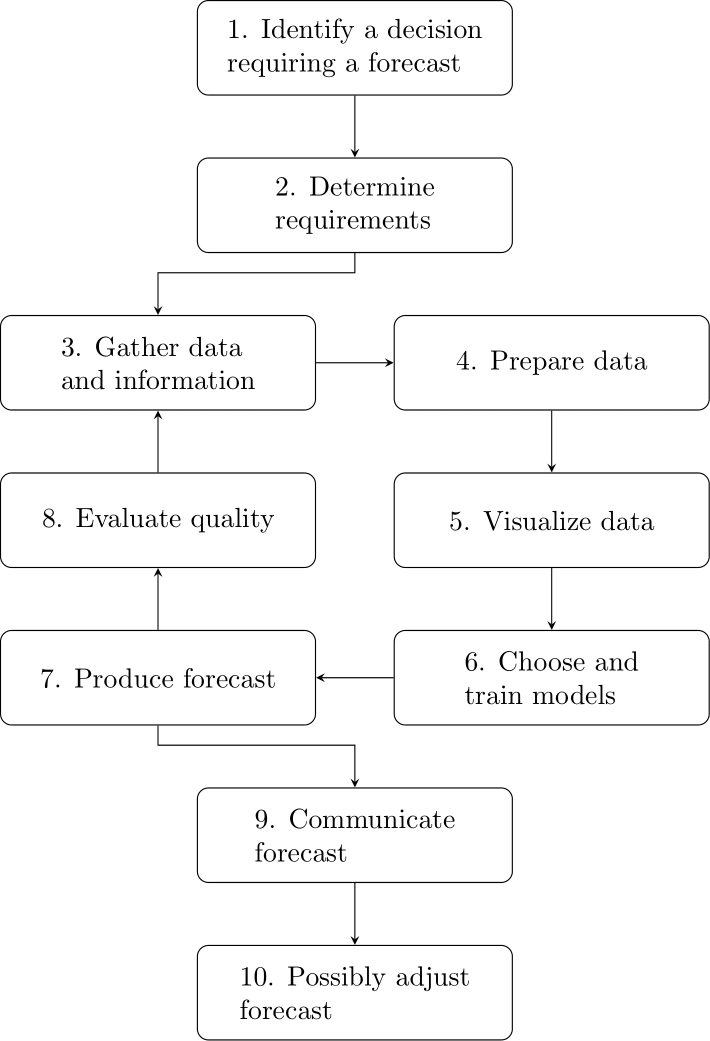
\includegraphics[width=2.37in,height=\textheight]{figs/forecasting_workflow.png}

}

\end{figure}
\end{frame}

\begin{frame}{Statistical forecasting steps}
\protect\hypertarget{statistical-forecasting-steps}{}
\begin{itemize}
\tightlist
\item
  Prepare data.
\item
  Visualise data.
\item
  Choosing and fitting models (specify and train models).
\item
  Produce forecast.
\item
  Evaluate quality.
\end{itemize}
\end{frame}

\begin{frame}{What is a forecast?}
\protect\hypertarget{what-is-a-forecast}{}
\forecast\pause

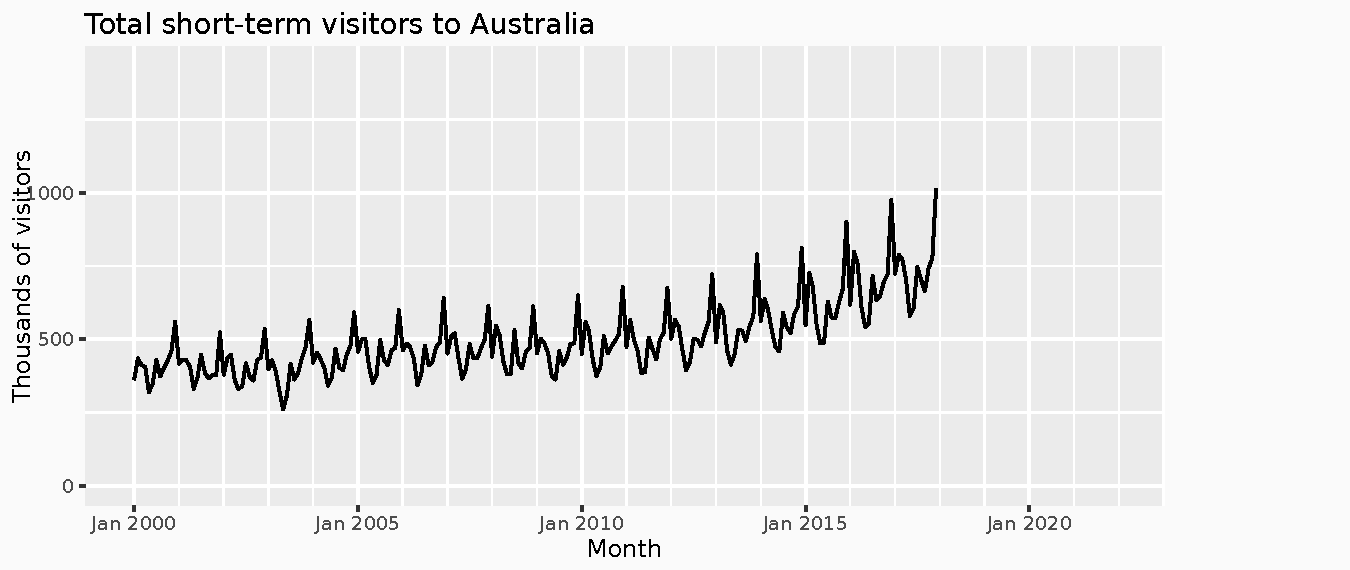
\includegraphics{03_basic_modelling_files/figure-beamer/austa1-1.pdf}
\end{frame}

\begin{frame}{What is a forecast?}
\protect\hypertarget{what-is-a-forecast-1}{}
\forecast

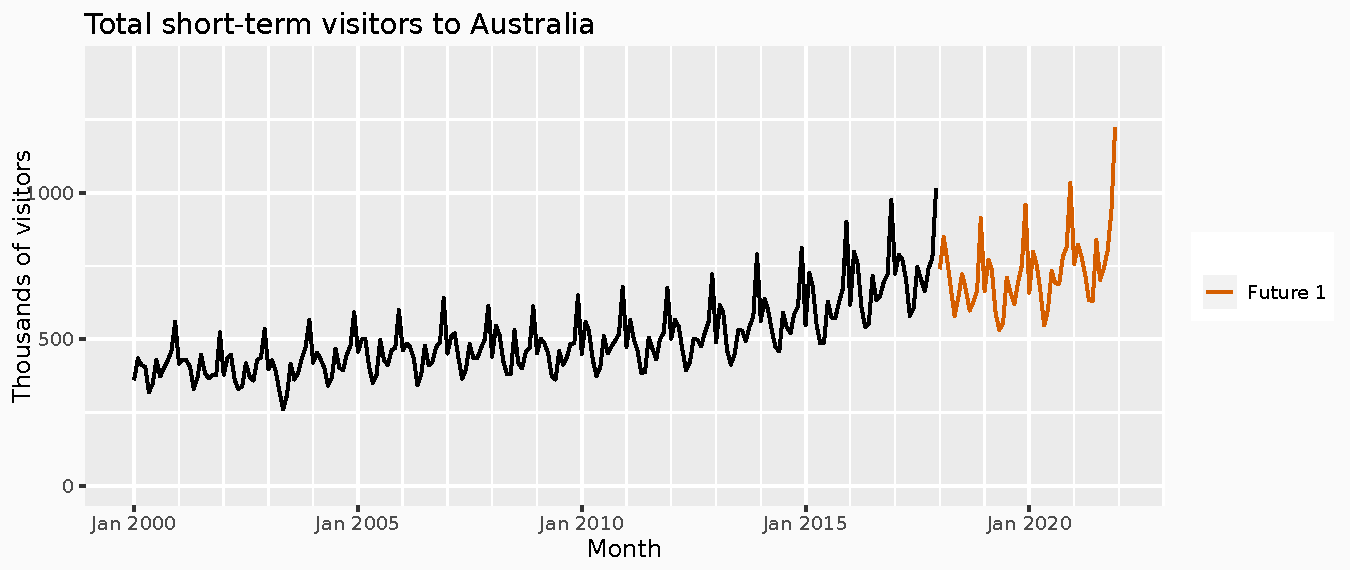
\includegraphics{03_basic_modelling_files/figure-beamer/austa2-1.pdf}

\simfutures
\end{frame}

\begin{frame}{What is a forecast?}
\protect\hypertarget{what-is-a-forecast-2}{}
\forecast

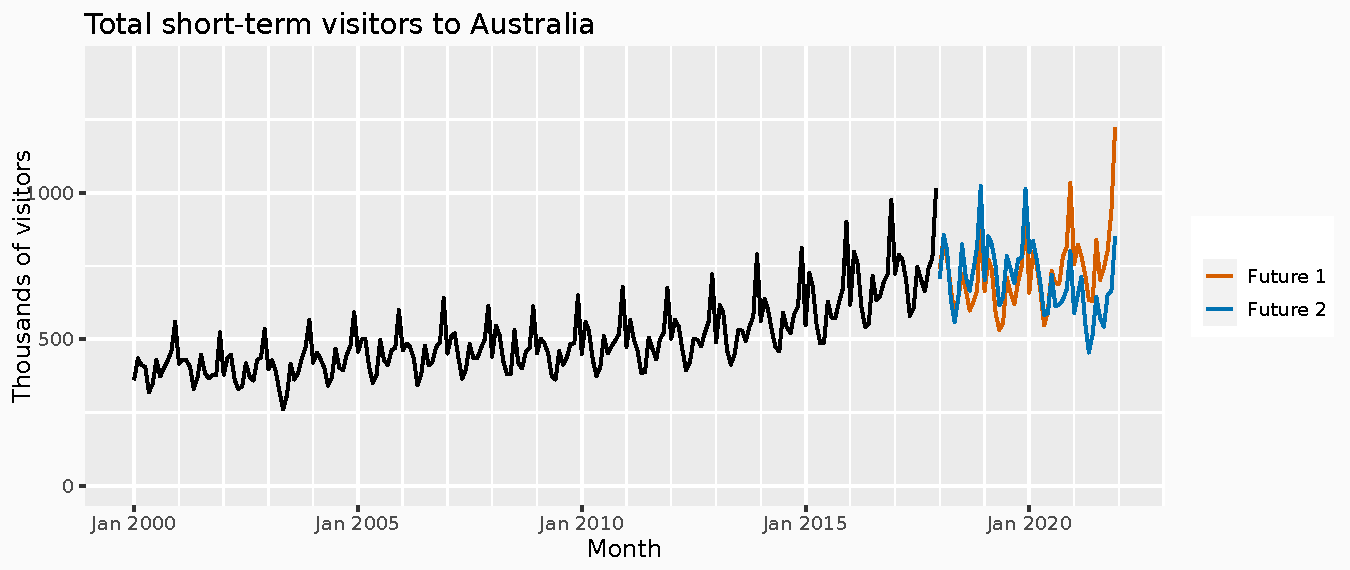
\includegraphics{03_basic_modelling_files/figure-beamer/austa3-1.pdf}

\simfutures
\end{frame}

\begin{frame}{What is a forecast?}
\protect\hypertarget{what-is-a-forecast-3}{}
\forecast

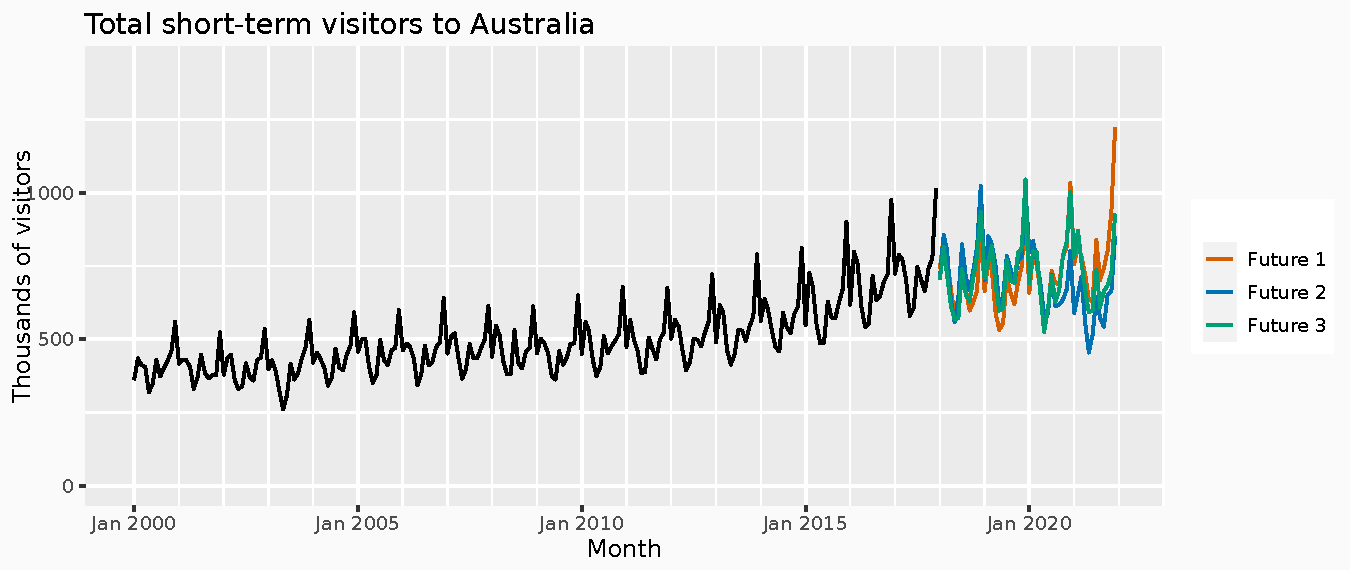
\includegraphics{03_basic_modelling_files/figure-beamer/austa4-1.pdf}

\simfutures
\end{frame}

\begin{frame}{What is a forecast?}
\protect\hypertarget{what-is-a-forecast-4}{}
\forecast

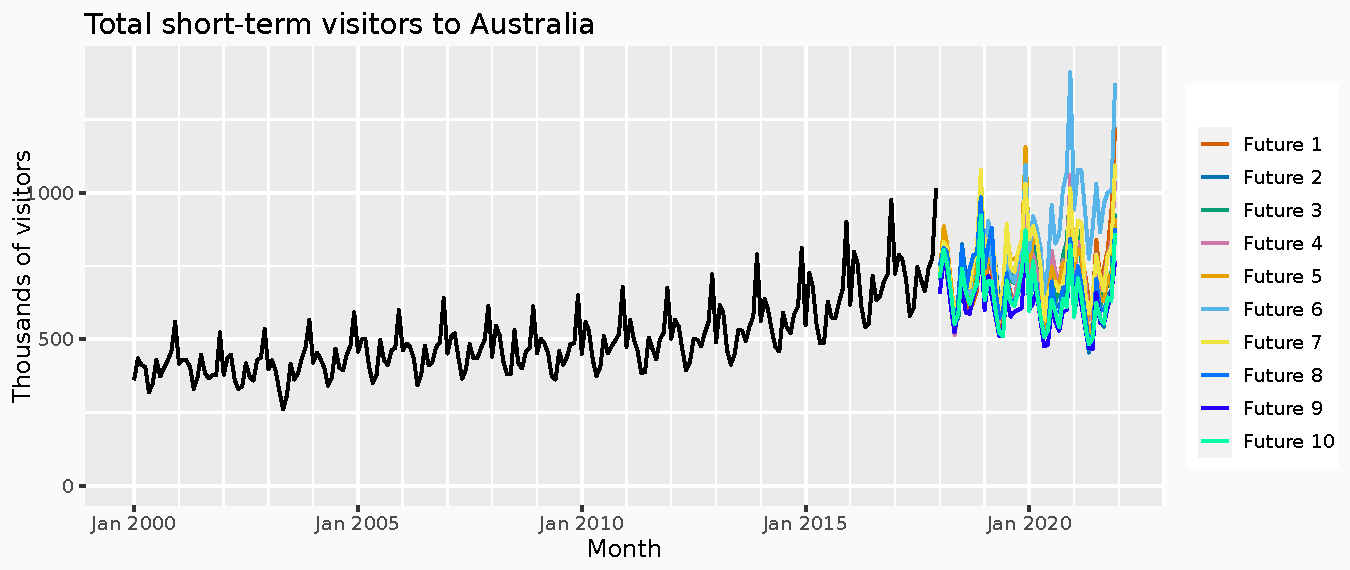
\includegraphics{03_basic_modelling_files/figure-beamer/austa5-1.pdf}

\simfutures
\end{frame}

\begin{frame}{What is a forecast?}
\protect\hypertarget{what-is-a-forecast-5}{}
\forecast

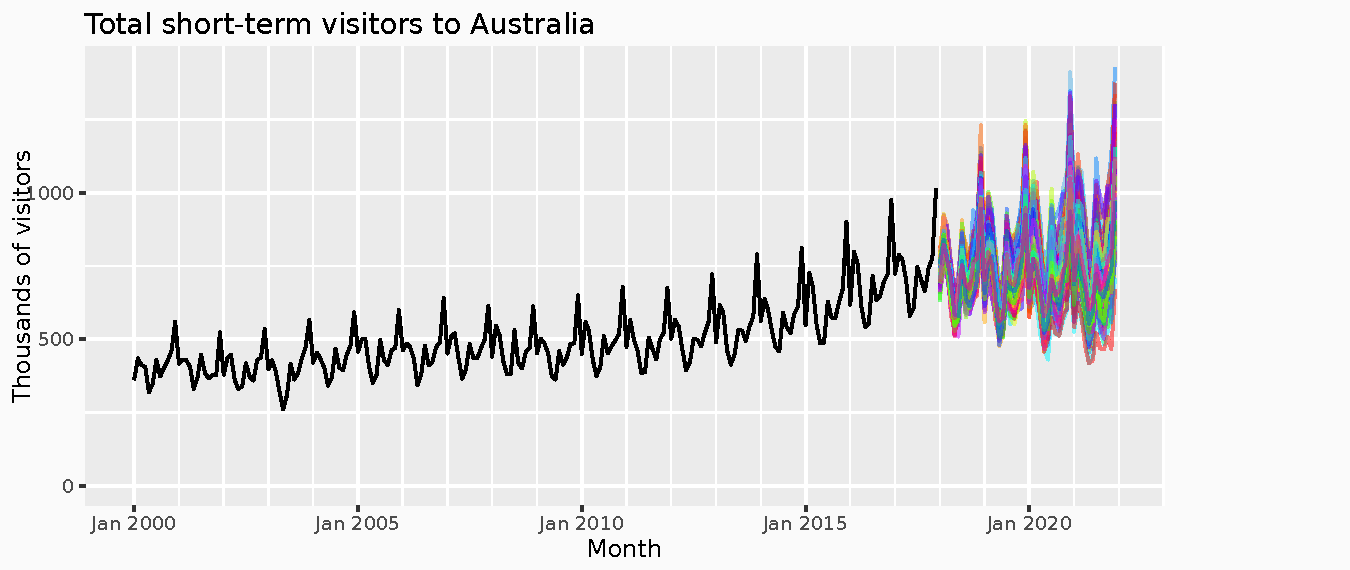
\includegraphics{03_basic_modelling_files/figure-beamer/austa6-1.pdf}

\simfutures
\end{frame}

\begin{frame}{What is a forecast?}
\protect\hypertarget{what-is-a-forecast-6}{}
\forecast

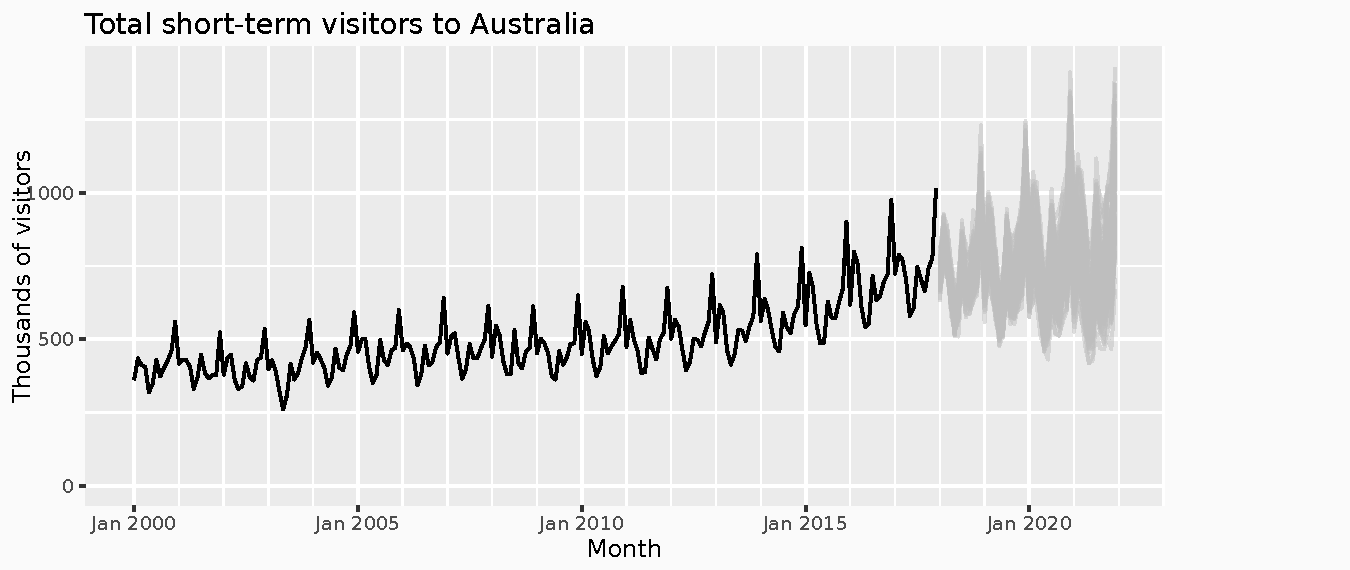
\includegraphics{03_basic_modelling_files/figure-beamer/austa7-1.pdf}

\simfutures
\end{frame}

\begin{frame}{What is a forecast?}
\protect\hypertarget{what-is-a-forecast-7}{}
\forecast

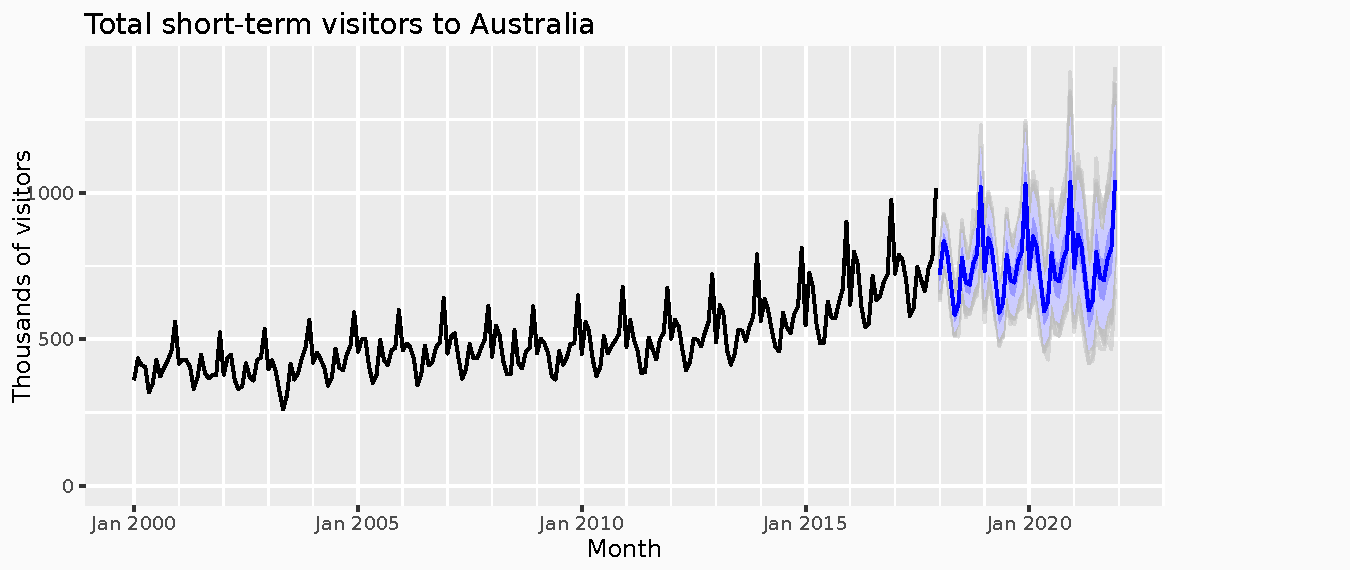
\includegraphics{03_basic_modelling_files/figure-beamer/austa8-1.pdf}

\simfutures
\end{frame}

\begin{frame}{Prediction interval}
\protect\hypertarget{prediction-interval}{}
\forecast

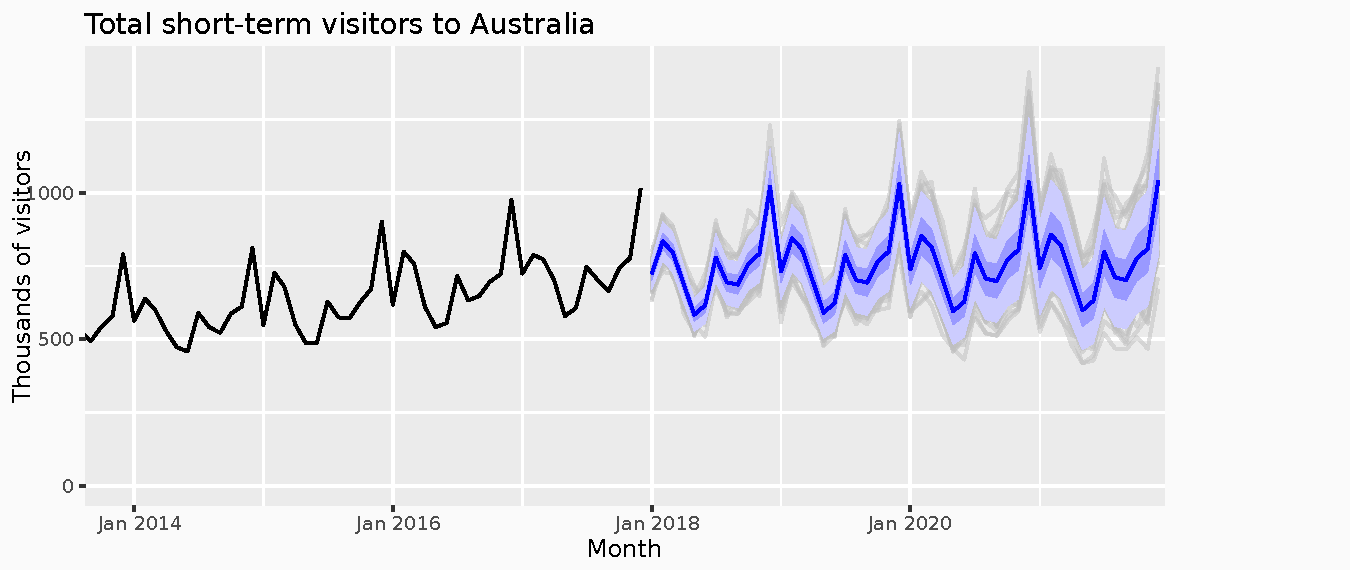
\includegraphics{03_basic_modelling_files/figure-beamer/austa9-1.pdf}

\simfutures
\end{frame}

\begin{frame}{Visualising forecast distributions}
\protect\hypertarget{visualising-forecast-distributions}{}
\begin{figure}

{\centering 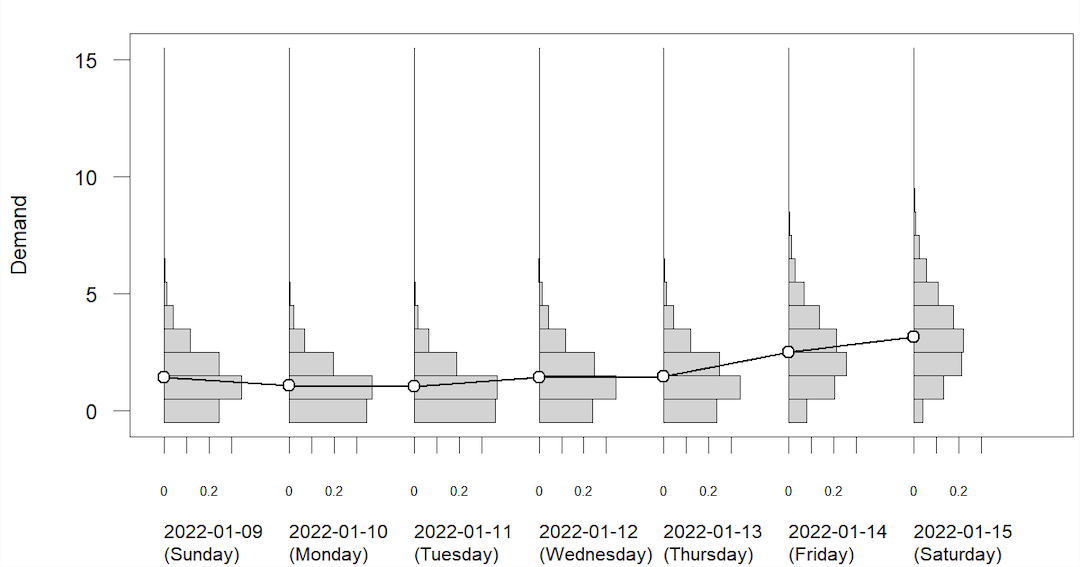
\includegraphics[width=0.7\textwidth,height=\textheight]{figs/daily_probabilistic_forecast.png}

}

\end{figure}
\end{frame}

\begin{frame}{Forecast distribution}
\protect\hypertarget{forecast-distribution}{}
\begin{figure}

{\centering 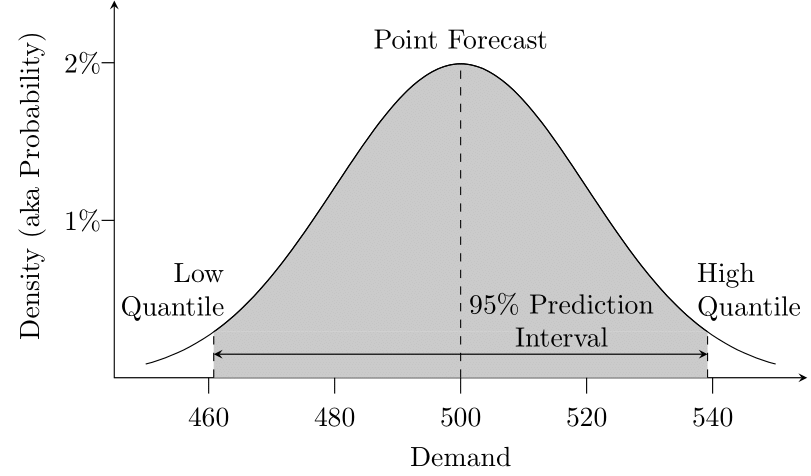
\includegraphics[width=0.7\textwidth,height=\textheight]{figs/forecasts_probabilistic_perspective.png}

}

\end{figure}
\end{frame}

\begin{frame}{Statistical forecasting}
\protect\hypertarget{statistical-forecasting-1}{}
\begin{itemize}
\tightlist
\item
  Thing to be forecast: \(y_{T+h}\).
\item
  What we know: \(y_1,\dots,y_T\).
\item
  Forecast distribution:
  \({y}_{T+h|t} = y_{T+h} \mid \{y_1,y_2,\dots,y_{T}\}\).
\item
  Point forecast:
  \(\hat{y}_{T+h|T} =\text{E}[y_{T+h} \mid y_1,\dots,y_T]\).
\item
  Forecast variance: \(\text{Var}[y_{t} \mid y_1,\dots,y_T]\)
\item
  Prediction interval is a range of values of \(y_{T+h}\) with high
  probability.
\end{itemize}
\end{frame}

\hypertarget{what-can-we-forecast}{%
\section{What can we forecast?}\label{what-can-we-forecast}}

\begin{frame}{What can we forecast?}
\protect\hypertarget{what-can-we-forecast-1}{}
\forecast

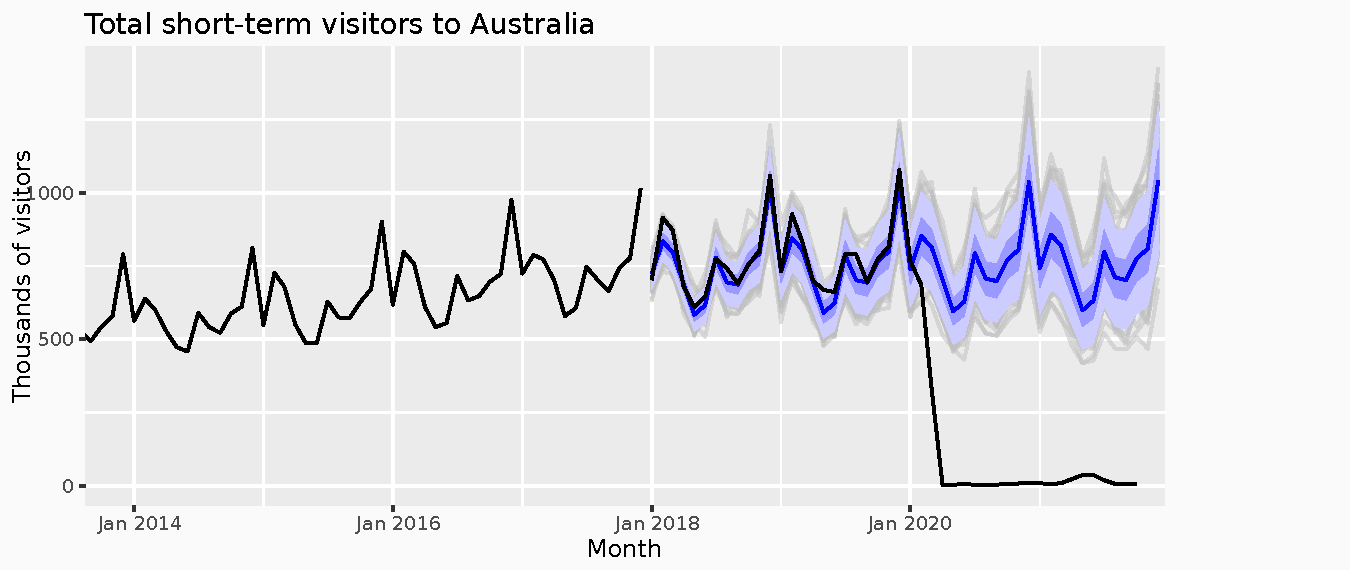
\includegraphics{03_basic_modelling_files/figure-beamer/austa9b-1.pdf}

\simfutures
\end{frame}

\begin{frame}{What can we forecast?}
\protect\hypertarget{what-can-we-forecast-2}{}
\full{nasdaq-stock-market}
\end{frame}

\begin{frame}{What can we forecast?}
\protect\hypertarget{what-can-we-forecast-3}{}
\full{Forex2}
\end{frame}

\begin{frame}{What can we forecast?}
\protect\hypertarget{what-can-we-forecast-4}{}
\full{pills}
\end{frame}

\begin{frame}{What can we forecast?}
\protect\hypertarget{what-can-we-forecast-5}{}
\full{elecwires2}
\end{frame}

\begin{frame}{What can we forecast?}
\protect\hypertarget{what-can-we-forecast-6}{}
\full{AusBOM}
\end{frame}

\begin{frame}{What can we forecast?}
\protect\hypertarget{what-can-we-forecast-7}{}
\full{ts22015}
\end{frame}

\begin{frame}{What can we forecast?}
\protect\hypertarget{what-can-we-forecast-8}{}
\full{comet}
\end{frame}

\begin{frame}{Which is easiest to forecast?}
\protect\hypertarget{which-is-easiest-to-forecast}{}
\begin{enumerate}
\tightlist
\item
  daily electricity demand in 3 days time
\item
  timing of next Halley's comet appearance
\item
  time of sunrise this day next year
\item
  Google stock price tomorrow
\item
  Google stock price in 6 months time
\item
  maximum temperature tomorrow
\item
  exchange rate of \$US/AUS next week
\item
  total sales of drugs in Australian pharmacies next month
\end{enumerate}

\pause

\begin{itemize}
\tightlist
\item
  how do we measure ``easiest''?
\item
  what makes something easy/difficult to forecast?
\end{itemize}
\end{frame}

\begin{frame}{Factors affecting forecastability}
\protect\hypertarget{factors-affecting-forecastability}{}
Something is easier to forecast if:

\begin{itemize}
\tightlist
\item
  we have a good understanding of the factors that contribute to it
\item
  there is lots of data available;
\item
  the forecasts cannot affect the thing we are trying to forecast.
\item
  there is relatively low natural/unexplainable random variation.
\item
  the future is somewhat similar to the past
\end{itemize}
\end{frame}

\hypertarget{benchmark-methods}{%
\section{Benchmark methods}\label{benchmark-methods}}

\begin{frame}{Some simple forecasting methods}
\protect\hypertarget{some-simple-forecasting-methods}{}
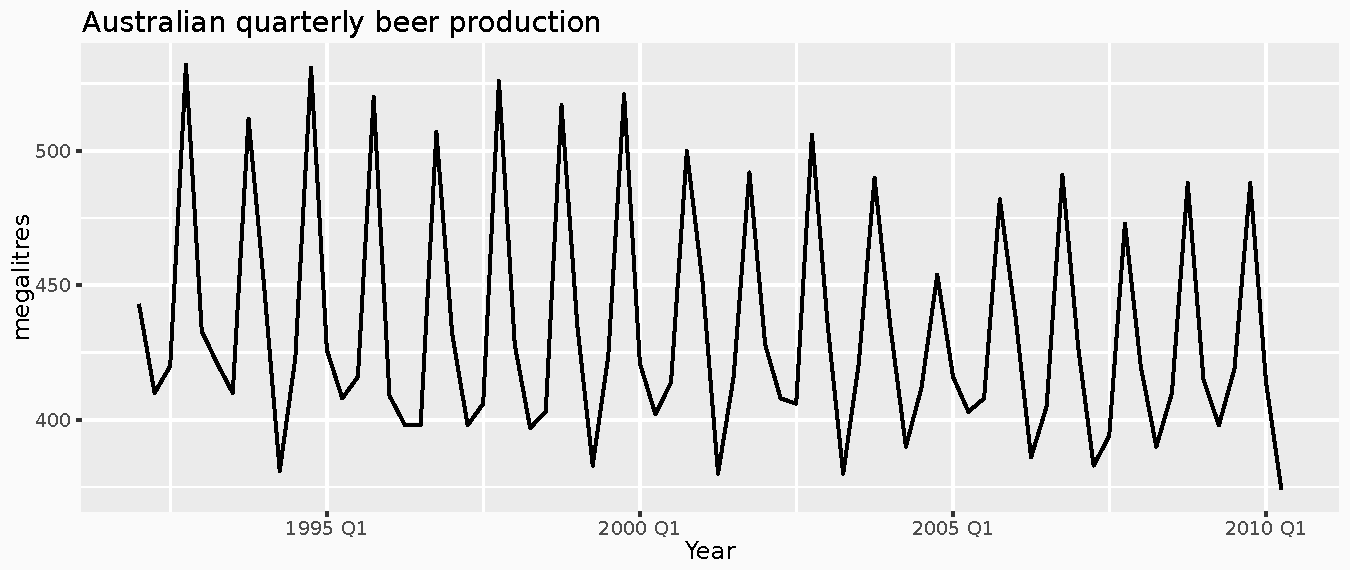
\includegraphics[width=0.9\textwidth,height=\textheight]{03_basic_modelling_files/figure-beamer/ausbeer-1.pdf}

\begin{textblock}{7}(0.4,6.9)
\begin{alertblock}{}
\small{How would you forecast these series?}
\end{alertblock}
\end{textblock}
\end{frame}

\begin{frame}{Some simple forecasting methods}
\protect\hypertarget{some-simple-forecasting-methods-1}{}
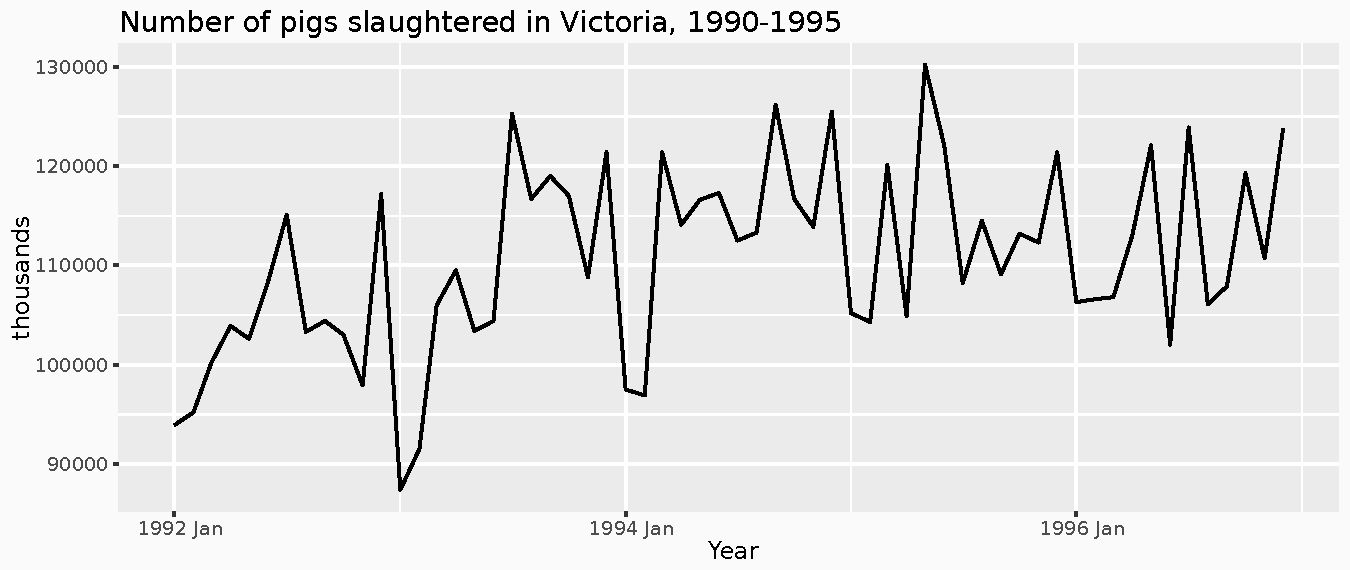
\includegraphics[width=0.9\textwidth,height=\textheight]{03_basic_modelling_files/figure-beamer/pigs-1.pdf}

\begin{textblock}{7}(0.4,6.9)
\begin{alertblock}{}
\small{How would you forecast these series?}
\end{alertblock}
\end{textblock}
\end{frame}

\begin{frame}{Some simple forecasting methods}
\protect\hypertarget{some-simple-forecasting-methods-2}{}
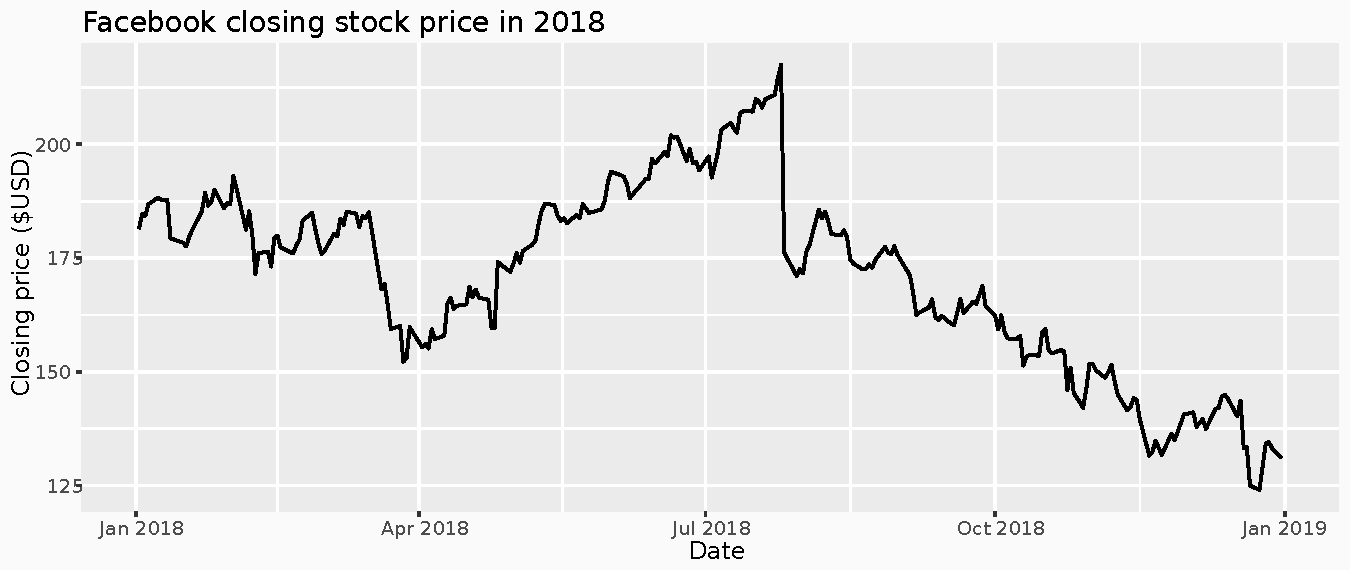
\includegraphics[width=0.9\textwidth,height=\textheight]{03_basic_modelling_files/figure-beamer/dj-1.pdf}

\begin{textblock}{7}(0.4,6.9)
\begin{alertblock}{}
\small{How would you forecast these series?}
\end{alertblock}
\end{textblock}
\end{frame}

\begin{frame}[fragile]{Some simple forecasting methods}
\protect\hypertarget{some-simple-forecasting-methods-3}{}
\fontsize{13}{14}\sf

\begin{block}{\texttt{MEAN(y)}: Average method}
\protect\hypertarget{meany-average-method}{}
\begin{itemize}
\tightlist
\item
  Forecast of all future values is equal to mean of historical data
  \(\{y_1,\dots,y_T\}\).
\item
  Forecasts: \(\hat{y}_{T+h|T} = \bar{y} = (y_1+\dots+y_T)/T\)
\end{itemize}

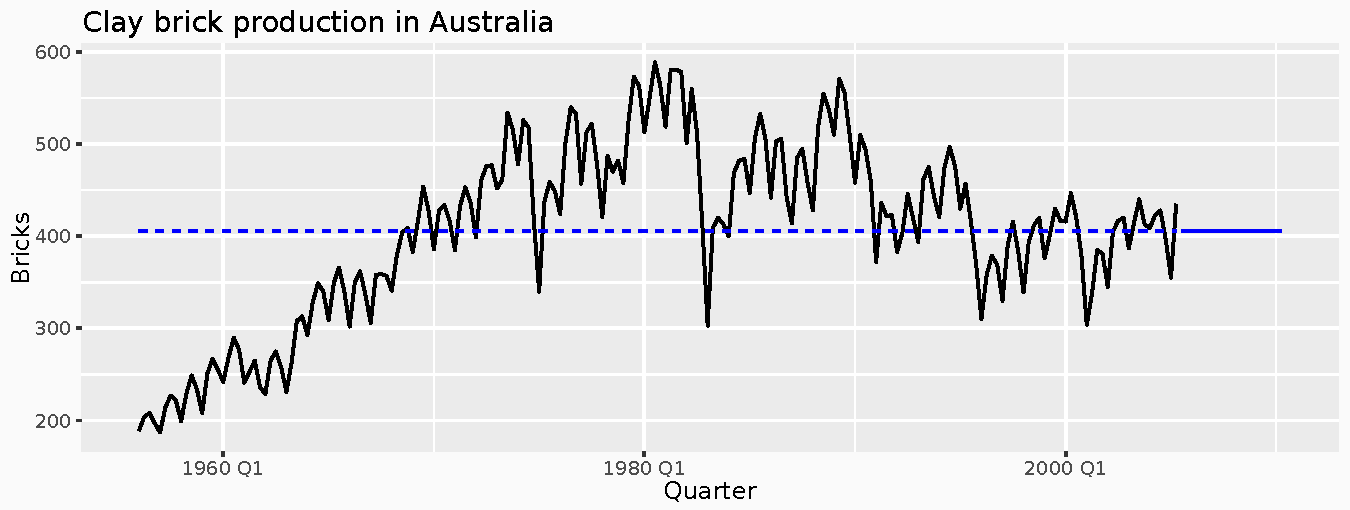
\includegraphics{03_basic_modelling_files/figure-beamer/mean-method-explained-1.pdf}
\end{block}
\end{frame}

\begin{frame}[fragile]{Some simple forecasting methods}
\protect\hypertarget{some-simple-forecasting-methods-4}{}
\fontsize{13}{14}\sf

\begin{block}{\texttt{NAIVE(y)}: Naïve method}
\protect\hypertarget{naivey-nauxefve-method}{}
\begin{itemize}
\tightlist
\item
  Forecasts equal to last observed value.
\item
  Forecasts: \(\hat{y}_{T+h|T} =y_T\).
\item
  Consequence of efficient market hypothesis.
\end{itemize}

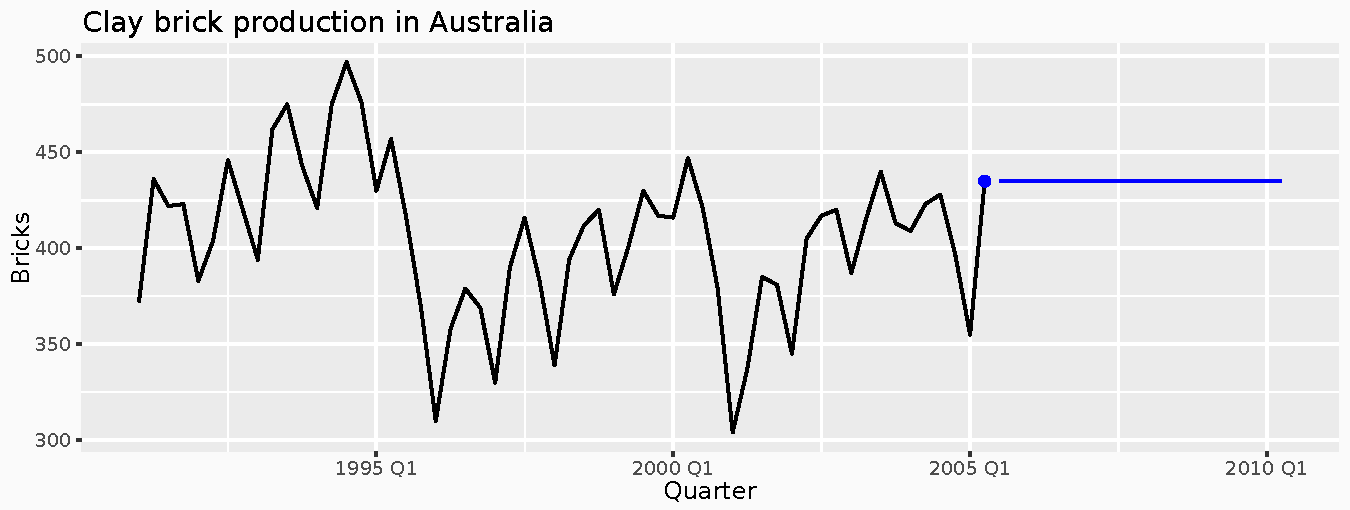
\includegraphics{03_basic_modelling_files/figure-beamer/naive-method-explained-1.pdf}
\end{block}
\end{frame}

\begin{frame}[fragile]{Some simple forecasting methods}
\protect\hypertarget{some-simple-forecasting-methods-5}{}
\fontsize{13}{14}\sf

\begin{block}{\texttt{SNAIVE(y\ \textasciitilde{}\ lag(m))}: Seasonal
naïve method}
\protect\hypertarget{snaivey-lagm-seasonal-nauxefve-method}{}
\begin{itemize}
\tightlist
\item
  Forecasts equal to last value from same season.
\item
  Forecasts: \(\hat{y}_{T+h|T} =y_{T+h-m(k+1)}\), where \(m=\) seasonal
  period and \(k\) is the integer part of \((h-1)/m\).
\end{itemize}

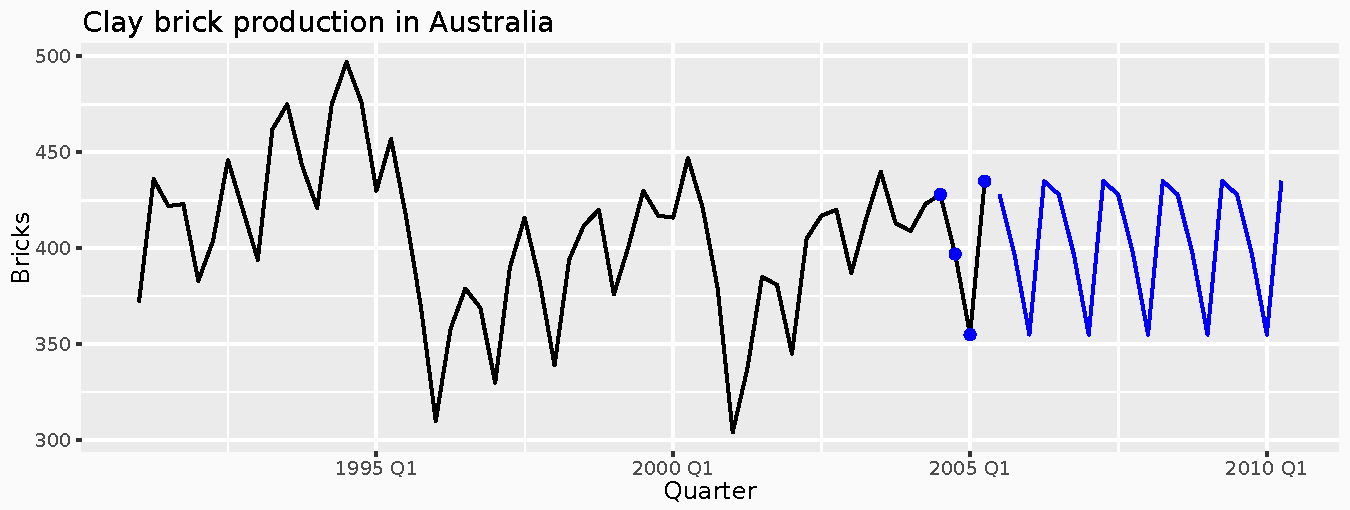
\includegraphics{03_basic_modelling_files/figure-beamer/snaive-method-explained-1.pdf}
\end{block}
\end{frame}

\begin{frame}[fragile]{Some simple forecasting methods}
\protect\hypertarget{some-simple-forecasting-methods-6}{}
\fontsize{13}{14}\sf

\begin{block}{\texttt{RW(y\ \textasciitilde{}\ drift())}: Drift method}
\protect\hypertarget{rwy-drift-drift-method}{}
\begin{itemize}
\tightlist
\item
  Forecasts equal to last value plus average change.
\item
  Forecasts:\vspace*{-.7cm}
\end{itemize}

\begin{align*}
 \hat{y}_{T+h|T} & =  y_{T} + \frac{h}{T-1}\sum_{t=2}^T (y_t-y_{t-1})\\
                 & = y_T + \frac{h}{T-1}(y_T -y_1).
 \end{align*}\vspace*{-0.2cm}

\begin{itemize}
\tightlist
\item
  Equivalent to extrapolating a line drawn between first and last
  observations.
\end{itemize}
\end{block}
\end{frame}

\begin{frame}{Some simple forecasting methods}
\protect\hypertarget{some-simple-forecasting-methods-7}{}
\begin{block}{Drift method}
\protect\hypertarget{drift-method}{}
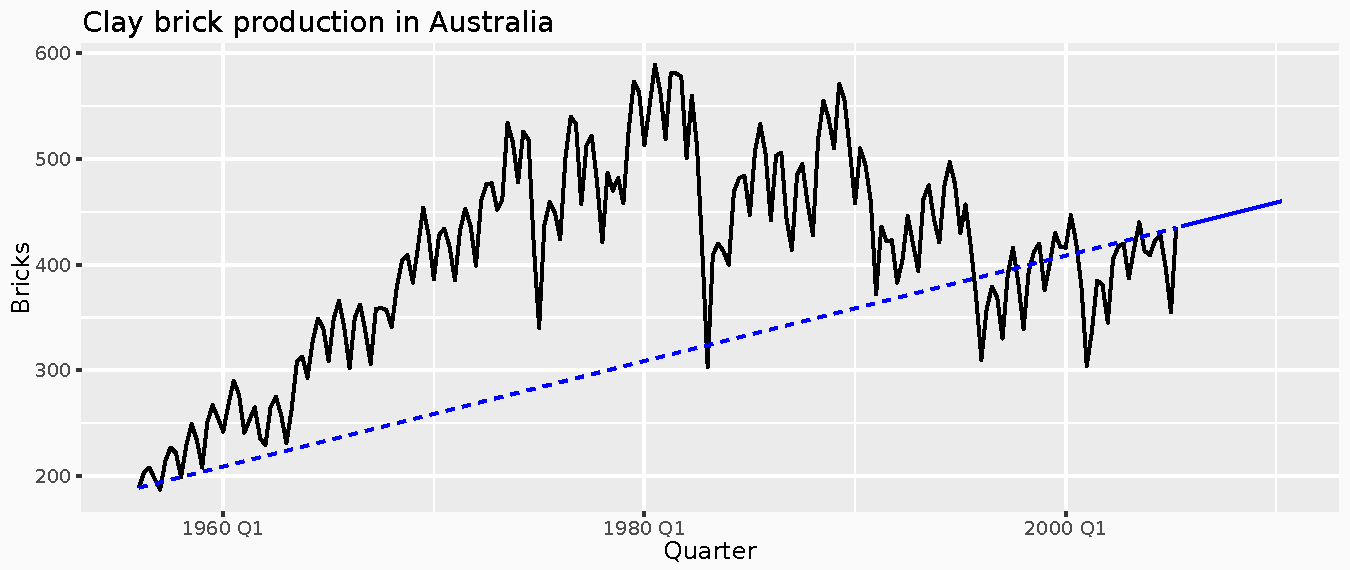
\includegraphics{03_basic_modelling_files/figure-beamer/drift-method-explained-1.pdf}
\end{block}
\end{frame}

\hypertarget{specify-and-estimate}{%
\section{Specify and estimate}\label{specify-and-estimate}}

\begin{frame}[fragile]{Model specification}
\protect\hypertarget{model-specification}{}
\begin{itemize}
\tightlist
\item
  Model specification in fable supports a formula based interface
\item
  A model formula in R is expressed using
  \texttt{response\ \textasciitilde{}\ terms}

  \begin{itemize}
  \tightlist
  \item
    the formula's left side describes the response
  \item
    the right describes terms used to model the response.
  \end{itemize}
\item
  \texttt{Attention}: MODEL name is in capital letters,
  e.g.~\texttt{SNAIVE}
\end{itemize}
\end{frame}

\begin{frame}[fragile]{Model estimation}
\protect\hypertarget{model-estimation}{}
The \texttt{model()} function trains models on data. - It returns a
\texttt{mable} object.

\fontsize{10}{13}\sf

\begin{Shaded}
\begin{Highlighting}[]
\CommentTok{\# Fit the models}
\NormalTok{my\_mable }\OtherTok{\textless{}{-}}\NormalTok{ my\_data }\SpecialCharTok{\%\textgreater{}\%}
  \FunctionTok{model}\NormalTok{(}
    \AttributeTok{choose\_name1 =} \FunctionTok{MODEL1}\NormalTok{(response }\SpecialCharTok{\textasciitilde{}}\NormalTok{ term1}\SpecialCharTok{+}\NormalTok{...),}
    \AttributeTok{choose\_name2 =} \FunctionTok{MODEL2}\NormalTok{(response }\SpecialCharTok{\textasciitilde{}}\NormalTok{ term1}\SpecialCharTok{+}\NormalTok{...),}
    \AttributeTok{choose\_name3 =} \FunctionTok{MODEL3}\NormalTok{(response }\SpecialCharTok{\textasciitilde{}}\NormalTok{ term1}\SpecialCharTok{+}\NormalTok{...),}
    \AttributeTok{choose\_name4 =} \FunctionTok{MODEL4}\NormalTok{(response }\SpecialCharTok{\textasciitilde{}}\NormalTok{ term1}\SpecialCharTok{+}\NormalTok{...)}
\NormalTok{  )}
\end{Highlighting}
\end{Shaded}
\end{frame}

\begin{frame}[fragile]{Model fitting- example}
\protect\hypertarget{model-fitting--example}{}
The \texttt{model()} function trains models on data.

\fontsize{10}{11}\sf

\begin{Shaded}
\begin{Highlighting}[]
\NormalTok{beer\_fit }\OtherTok{\textless{}{-}}\NormalTok{ aus\_production }\SpecialCharTok{|\textgreater{}}
  \FunctionTok{model}\NormalTok{(}
    \StringTok{\textasciigrave{}}\AttributeTok{Seasonal\_naïve}\StringTok{\textasciigrave{}} \OtherTok{=} \FunctionTok{SNAIVE}\NormalTok{(Beer),}
    \StringTok{\textasciigrave{}}\AttributeTok{Naïve}\StringTok{\textasciigrave{}} \OtherTok{=} \FunctionTok{NAIVE}\NormalTok{(Beer),}
    \AttributeTok{Drift =} \FunctionTok{RW}\NormalTok{(Beer }\SpecialCharTok{\textasciitilde{}} \FunctionTok{drift}\NormalTok{()),}
    \AttributeTok{Mean =} \FunctionTok{MEAN}\NormalTok{(Beer)}
\NormalTok{  )}
\end{Highlighting}
\end{Shaded}

\begin{verbatim}
# A mable: 1 x 4
  Seasonal_naïve   Naïve         Drift    Mean
         <model> <model>       <model> <model>
1       <SNAIVE> <NAIVE> <RW w/ drift>  <MEAN>
\end{verbatim}

\vspace*{0.2cm}\begin{alertblock}{}
A \texttt{mable} is a model table, each cell corresponds to a fitted model.
\end{alertblock}
\end{frame}

\begin{frame}[fragile]{Extract information from \texttt{mable}}
\protect\hypertarget{extract-information-from-mable}{}
\fontsize{10}{12}\sf

\begin{Shaded}
\begin{Highlighting}[]
\NormalTok{beer\_fit }\SpecialCharTok{\%\textgreater{}\%} \FunctionTok{select}\NormalTok{(snaive) }\SpecialCharTok{\%\textgreater{}\%} \FunctionTok{report}\NormalTok{()}
\NormalTok{beer\_fit }\SpecialCharTok{\%\textgreater{}\%} \FunctionTok{tidy}\NormalTok{()}
\NormalTok{beer\_fit }\SpecialCharTok{\%\textgreater{}\%} \FunctionTok{glance}\NormalTok{()}
\end{Highlighting}
\end{Shaded}

\begin{itemize}
\tightlist
\item
  The \texttt{report()} function gives a formatted model-specific
  display.
\item
  The \texttt{tidy()} function is used to extract the coefficients from
  the models.
\item
  We can extract information about some specific model using the
  \texttt{filter()} and \texttt{select()}functions.
\end{itemize}
\end{frame}

\begin{frame}{Check model performance}
\protect\hypertarget{check-model-performance}{}
Once a model has been fitted, it is important to check how well it has
performed on the data. I come back to this latter.
\end{frame}

\hypertarget{produce-forecasts}{%
\section{Produce forecasts}\label{produce-forecasts}}

\begin{frame}[fragile]{Producing forecasts}
\protect\hypertarget{producing-forecasts}{}
\begin{itemize}
\tightlist
\item
  The \texttt{forecast()} function is used to produce forecasts from
  estimated models.
\item
  \textbf{h} can be specified with:

  \begin{itemize}
  \tightlist
  \item
    a number (the number of future observations)
  \item
    natural language (the length of time to predict)
  \item
    provide a dataset of future time periods
  \end{itemize}
\end{itemize}
\end{frame}

\begin{frame}[fragile]{Producing forecasts}
\protect\hypertarget{producing-forecasts-1}{}
\fontsize{10}{13}\sf

\begin{Shaded}
\begin{Highlighting}[]
\NormalTok{beer\_fc }\OtherTok{\textless{}{-}}\NormalTok{ beer\_fit }\SpecialCharTok{|\textgreater{}}
  \FunctionTok{forecast}\NormalTok{(}\AttributeTok{h =} \StringTok{"5 years"}\NormalTok{)}
\end{Highlighting}
\end{Shaded}

\begin{verbatim}
# A fable: 80 x 4 [1Q]
# Key:     .model [4]
  .model         Quarter        Beer .mean
  <chr>            <qtr>      <dist> <dbl>
1 Seasonal_naïve 2010 Q3 N(419, 373)   419
2 Seasonal_naïve 2010 Q4 N(488, 373)   488
3 Seasonal_naïve 2011 Q1 N(414, 373)   414
4 Seasonal_naïve 2011 Q2 N(374, 373)   374
# i 76 more rows
\end{verbatim}

\vspace*{0.2cm}\begin{alertblock}{}
A \texttt{fable} is a forecast table with point forecasts and distributions.
\end{alertblock}
\end{frame}

\begin{frame}[fragile]{Visualising forecasts}
\protect\hypertarget{visualising-forecasts}{}
\footnotesize

\begin{Shaded}
\begin{Highlighting}[]
\NormalTok{beer\_fc }\SpecialCharTok{|\textgreater{}}
  \FunctionTok{autoplot}\NormalTok{(aus\_production, }\AttributeTok{level =} \ConstantTok{NULL}\NormalTok{) }\SpecialCharTok{+}
  \FunctionTok{labs}\NormalTok{(}\AttributeTok{title =} \StringTok{"Forecasts for quarterly clay brick production"}\NormalTok{,}
       \AttributeTok{x =} \StringTok{"Year"}\NormalTok{, }\AttributeTok{y =} \StringTok{"Millions of bricks"}\NormalTok{) }\SpecialCharTok{+}
  \FunctionTok{guides}\NormalTok{(}\AttributeTok{colour =} \FunctionTok{guide\_legend}\NormalTok{(}\AttributeTok{title =} \StringTok{"Forecast"}\NormalTok{))}
\end{Highlighting}
\end{Shaded}

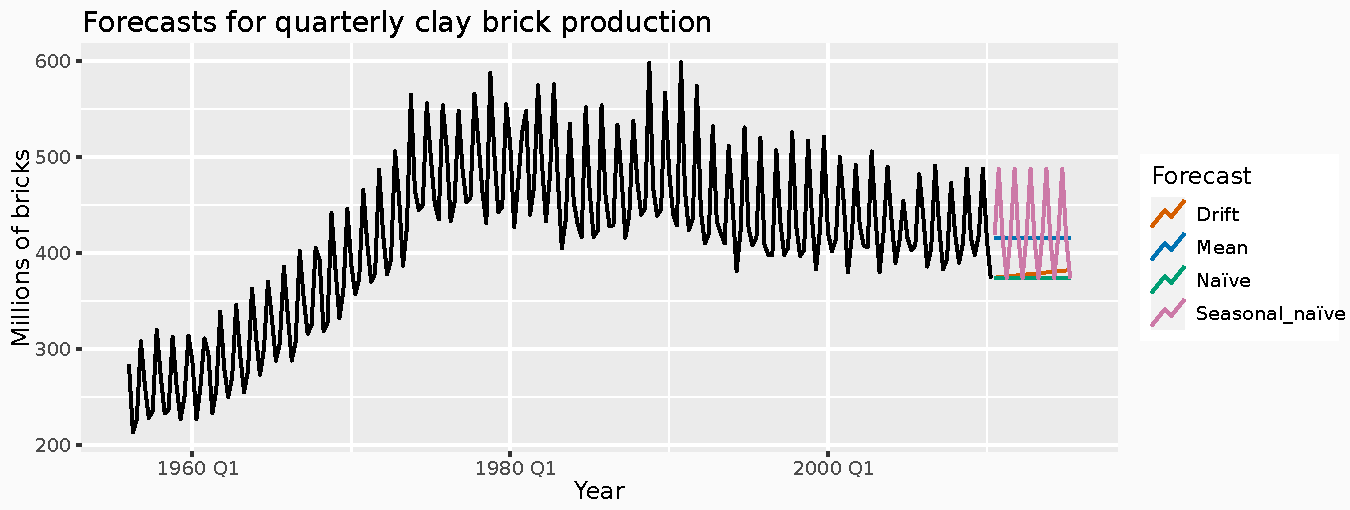
\includegraphics{03_basic_modelling_files/figure-beamer/beer-fc-plot-1.pdf}
\end{frame}

\begin{frame}{Forecast distributions}
\protect\hypertarget{forecast-distributions}{}
\begin{itemize}
\tightlist
\item
  A forecast \(\hat{y}_{T+h|T}\) is (usually) the mean of the
  conditional distribution \(y_{T+h} \mid y_1, \dots, y_{T}\).
\item
  Most time series models produce normally distributed forecasts.
\item
  The forecast distribution describes the probability of observing any
  future value.
\end{itemize}
\end{frame}

\begin{frame}{Forecast distributions - normal distribution}
\protect\hypertarget{forecast-distributions---normal-distribution}{}
\fontsize{14}{18}\sf

Assuming residuals are normal, uncorrelated, sd = \(\hat\sigma\):

\begin{block}{}
\begin{tabular}{ll}
\bf Mean: & $\hat{y}_{T+h|T} \sim N(\bar{y}, (1 + 1/T)\hat{\sigma}^2)$\\[0.2cm]
\bf Naïve: & $\hat{y}_{T+h|T} \sim N(y_T, h\hat{\sigma}^2)$\\[0.2cm]
\bf Seasonal naïve: & $\hat{y}_{T+h|T} \sim N(y_{T+h-m(k+1)}, (k+1)\hat{\sigma}^2)$\\[0.2cm]
\bf Drift: & $\hat{y}_{T+h|T} \sim N(y_T + \frac{h}{T-1}(y_T - y_1),h\frac{T+h}{T}\hat{\sigma}^2)$
\end{tabular}
\end{block}

where \(k\) is the integer part of \((h-1)/m\).

Note that when \(h=1\) and \(T\) is large, these all give the same
approximate forecast variance: \(\hat{\sigma}^2\).
\end{frame}

\begin{frame}{Forecast distributions from bootstrapping}
\protect\hypertarget{forecast-distributions-from-bootstrapping}{}
\fontsize{10}{13}\sf

When a normal distribution for the residuals is an unreasonable
assumption, one alternative is to use bootstrapping, which only assumes
that the residuals are uncorrelated with constant variance.

\begin{itemize}
\item
  A one-step forecast error is defined as
  \(e_t = y_t - \hat{y}_{t|t-1}\), \(y_t = \hat{y}_{t|t-1} + e_t.\)
\item
  So we can simulate the next observation of a time series using
  \(y_{T+1} = \hat{y}_{T+1|T} + e_{T+1}\)
\item
  Adding the new simulated observation to our data set, we can repeat
  the process to obtain \(y_{T+2} = \hat{y}_{T+2|T+1} + e_{T+2}\)
\end{itemize}
\end{frame}

\begin{frame}[fragile]{Generate many possible future using
\texttt{generate()}}
\protect\hypertarget{generate-many-possible-future-using-generate}{}
\fontsize{10}{13}\sf

\begin{Shaded}
\begin{Highlighting}[]
\NormalTok{beer\_2000 }\OtherTok{\textless{}{-}}\NormalTok{ aus\_production }\SpecialCharTok{|\textgreater{}} \FunctionTok{filter}\NormalTok{(}\FunctionTok{year}\NormalTok{(Quarter) }\SpecialCharTok{==} \DecValTok{2000}\NormalTok{) }\SpecialCharTok{|\textgreater{}} \FunctionTok{select}\NormalTok{(Beer)}
\NormalTok{fit }\OtherTok{\textless{}{-}}\NormalTok{ beer\_2000 }\SpecialCharTok{|\textgreater{}}
  \FunctionTok{model}\NormalTok{(}\FunctionTok{NAIVE}\NormalTok{(Beer))}
\NormalTok{sim }\OtherTok{\textless{}{-}}\NormalTok{ fit }\SpecialCharTok{|\textgreater{}} \FunctionTok{generate}\NormalTok{(}\AttributeTok{h =} \DecValTok{12}\NormalTok{, }\AttributeTok{times =} \DecValTok{5}\NormalTok{, }\AttributeTok{bootstrap =} \ConstantTok{TRUE}\NormalTok{)}
\NormalTok{sim}
\end{Highlighting}
\end{Shaded}

\begin{verbatim}
# A tsibble: 60 x 5 [1Q]
# Key:       .model, .rep [5]
   .model      .rep  Quarter .innov  .sim
   <chr>       <chr>   <qtr>  <dbl> <dbl>
 1 NAIVE(Beer) 1     2001 Q1  -45.3  455.
 2 NAIVE(Beer) 1     2001 Q2  -45.3  409.
 3 NAIVE(Beer) 1     2001 Q3  -14.3  395 
 4 NAIVE(Beer) 1     2001 Q4  -14.3  381.
 5 NAIVE(Beer) 1     2002 Q1  -45.3  335.
 6 NAIVE(Beer) 1     2002 Q2  -14.3  321 
 7 NAIVE(Beer) 1     2002 Q3   59.7  381.
 8 NAIVE(Beer) 1     2002 Q4   59.7  440.
 9 NAIVE(Beer) 1     2003 Q1  -14.3  426 
10 NAIVE(Beer) 1     2003 Q2  -45.3  381.
# i 50 more rows
\end{verbatim}
\end{frame}

\begin{frame}{Generate 5 different futures}
\protect\hypertarget{generate-5-different-futures}{}
\fontsize{10}{13}\sf

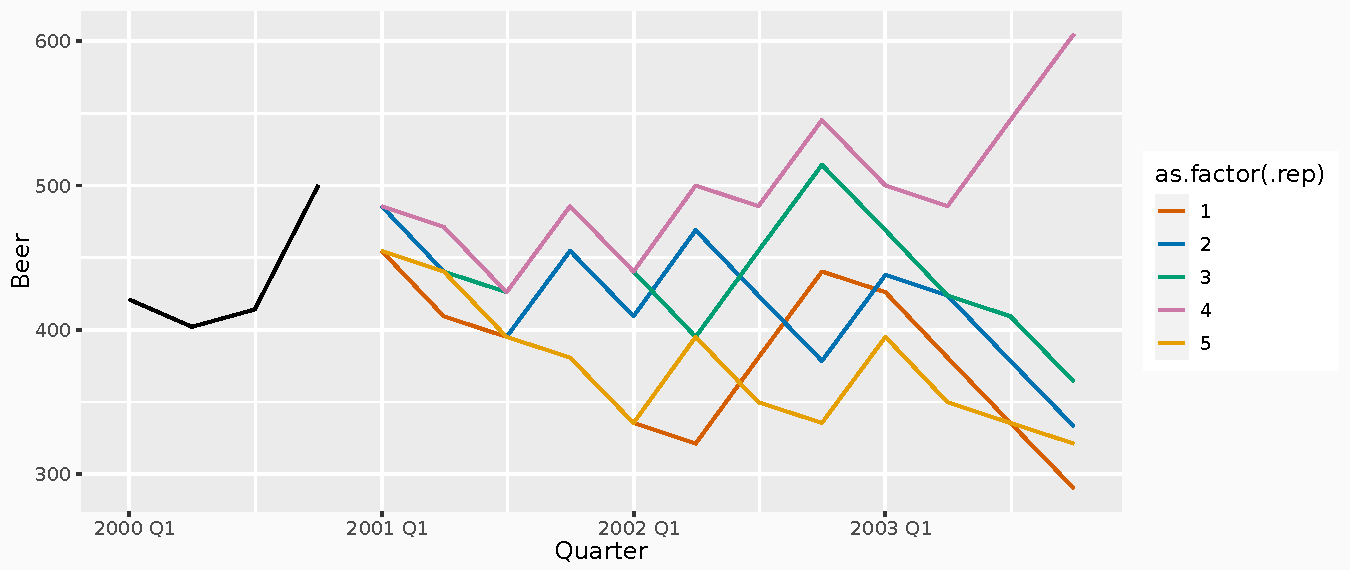
\includegraphics{03_basic_modelling_files/figure-beamer/visualise-future-1.pdf}
\end{frame}

\begin{frame}[fragile]{Use \texttt{forecast()} function to generate
probabilistic forecasts}
\protect\hypertarget{use-forecast-function-to-generate-probabilistic-forecasts}{}
\fontsize{10}{13}\sf

\begin{Shaded}
\begin{Highlighting}[]
\NormalTok{fc }\OtherTok{\textless{}{-}}\NormalTok{ fit }\SpecialCharTok{|\textgreater{}} \FunctionTok{forecast}\NormalTok{(}\AttributeTok{h =} \DecValTok{12}\NormalTok{, }\AttributeTok{bootstrap =} \ConstantTok{TRUE}\NormalTok{)}
\NormalTok{fc}
\end{Highlighting}
\end{Shaded}

\begin{verbatim}
# A fable: 12 x 4 [1Q]
# Key:     .model [1]
   .model      Quarter         Beer .mean
   <chr>         <qtr>       <dist> <dbl>
 1 NAIVE(Beer) 2001 Q1 sample[5000]  500.
 2 NAIVE(Beer) 2001 Q2 sample[5000]  500.
 3 NAIVE(Beer) 2001 Q3 sample[5000]  500.
 4 NAIVE(Beer) 2001 Q4 sample[5000]  499.
 5 NAIVE(Beer) 2002 Q1 sample[5000]  500.
 6 NAIVE(Beer) 2002 Q2 sample[5000]  500.
 7 NAIVE(Beer) 2002 Q3 sample[5000]  500.
 8 NAIVE(Beer) 2002 Q4 sample[5000]  500.
 9 NAIVE(Beer) 2003 Q1 sample[5000]  499.
10 NAIVE(Beer) 2003 Q2 sample[5000]  500.
11 NAIVE(Beer) 2003 Q3 sample[5000]  500.
12 NAIVE(Beer) 2003 Q4 sample[5000]  499.
\end{verbatim}
\end{frame}

\begin{frame}{Prediction intervals}
\protect\hypertarget{prediction-intervals}{}
\begin{itemize}
\tightlist
\item
  A prediction interval gives a region within which we expect
  \(y_{T+h}\) to lie with a specified probability
\item
  It consists of an upper and a lower limit between which the future
  value is expected to lie
\end{itemize}
\end{frame}

\begin{frame}[fragile]{Prediction intervals}
\protect\hypertarget{prediction-intervals-1}{}
\begin{itemize}
\tightlist
\item
  Forecast intervals can be extracted using the \texttt{hilo()}
  function.
\end{itemize}

\fontsize{10}{13}\sf

\begin{Shaded}
\begin{Highlighting}[]
\NormalTok{fit }\OtherTok{\textless{}{-}}\NormalTok{ aus\_production }\SpecialCharTok{|\textgreater{}} \FunctionTok{select}\NormalTok{(Beer) }\SpecialCharTok{\%\textgreater{}\%} \FunctionTok{model}\NormalTok{(}\FunctionTok{NAIVE}\NormalTok{(Beer))}
\FunctionTok{forecast}\NormalTok{(fit) }\SpecialCharTok{\%\textgreater{}\%} \FunctionTok{hilo}\NormalTok{(}\AttributeTok{level =} \DecValTok{95}\NormalTok{) }\SpecialCharTok{\%\textgreater{}\%} \FunctionTok{unpack\_hilo}\NormalTok{(}\StringTok{"95\%"}\NormalTok{)}
\end{Highlighting}
\end{Shaded}

\begin{verbatim}
# A tsibble: 8 x 6 [1Q]
# Key:       .model [1]
  .model      Quarter          Beer .mean `95%_lower` `95%_upper`
  <chr>         <qtr>        <dist> <dbl>       <dbl>       <dbl>
1 NAIVE(Beer) 2010 Q3  N(374, 4580)   374      241.          507.
2 NAIVE(Beer) 2010 Q4  N(374, 9159)   374      186.          562.
3 NAIVE(Beer) 2011 Q1 N(374, 13739)   374      144.          604.
4 NAIVE(Beer) 2011 Q2 N(374, 18319)   374      109.          639.
5 NAIVE(Beer) 2011 Q3 N(374, 22898)   374       77.4         671.
6 NAIVE(Beer) 2011 Q4 N(374, 27478)   374       49.1         699.
7 NAIVE(Beer) 2012 Q1 N(374, 32057)   374       23.1         725.
8 NAIVE(Beer) 2012 Q2 N(374, 36637)   374       -1.15        749.
\end{verbatim}
\end{frame}

\begin{frame}[fragile]{Prediction intervals}
\protect\hypertarget{prediction-intervals-2}{}
\fontsize{10}{12}\sf

\begin{Shaded}
\begin{Highlighting}[]
\NormalTok{beer\_fc }\SpecialCharTok{|\textgreater{}}
  \FunctionTok{hilo}\NormalTok{(}\AttributeTok{level =} \FunctionTok{c}\NormalTok{(}\DecValTok{50}\NormalTok{, }\DecValTok{75}\NormalTok{))}
\end{Highlighting}
\end{Shaded}

\begin{verbatim}
# A tsibble: 80 x 6 [1Q]
# Key:       .model [4]
   .model         Quarter         Beer .mean        `50%`        `75%`
   <chr>            <qtr>       <dist> <dbl>       <hilo>       <hilo>
 1 Seasonal_naïve 2010 Q3  N(419, 373)   419 [406, 432]50 [397, 441]75
 2 Seasonal_naïve 2010 Q4  N(488, 373)   488 [475, 501]50 [466, 510]75
 3 Seasonal_naïve 2011 Q1  N(414, 373)   414 [401, 427]50 [392, 436]75
 4 Seasonal_naïve 2011 Q2  N(374, 373)   374 [361, 387]50 [352, 396]75
 5 Seasonal_naïve 2011 Q3  N(419, 747)   419 [401, 437]50 [388, 450]75
 6 Seasonal_naïve 2011 Q4  N(488, 747)   488 [470, 506]50 [457, 519]75
 7 Seasonal_naïve 2012 Q1  N(414, 747)   414 [396, 432]50 [383, 445]75
 8 Seasonal_naïve 2012 Q2  N(374, 747)   374 [356, 392]50 [343, 405]75
 9 Seasonal_naïve 2012 Q3 N(419, 1120)   419 [396, 442]50 [380, 458]75
10 Seasonal_naïve 2012 Q4 N(488, 1120)   488 [465, 511]50 [449, 527]75
# i 70 more rows
\end{verbatim}
\end{frame}

\begin{frame}[fragile]{Prediction intervals}
\protect\hypertarget{prediction-intervals-3}{}
\fontsize{10}{12}\sf

\begin{Shaded}
\begin{Highlighting}[]
\NormalTok{beer\_fc }\SpecialCharTok{|\textgreater{}}
  \FunctionTok{hilo}\NormalTok{(}\AttributeTok{level =} \FunctionTok{c}\NormalTok{(}\DecValTok{50}\NormalTok{, }\DecValTok{75}\NormalTok{)) }\SpecialCharTok{|\textgreater{}}
  \FunctionTok{mutate}\NormalTok{(}\AttributeTok{lower =} \StringTok{\textasciigrave{}}\AttributeTok{50\%}\StringTok{\textasciigrave{}}\SpecialCharTok{$}\NormalTok{lower, }\AttributeTok{upper =} \StringTok{\textasciigrave{}}\AttributeTok{50\%}\StringTok{\textasciigrave{}}\SpecialCharTok{$}\NormalTok{upper)}
\end{Highlighting}
\end{Shaded}

\begin{verbatim}
# A tsibble: 80 x 8 [1Q]
# Key:       .model [4]
   .model         Quarter         Beer .mean        `50%`        `75%` lower upper
   <chr>            <qtr>       <dist> <dbl>       <hilo>       <hilo> <dbl> <dbl>
 1 Seasonal_naïve 2010 Q3  N(419, 373)   419 [406, 432]50 [397, 441]75  406.  432.
 2 Seasonal_naïve 2010 Q4  N(488, 373)   488 [475, 501]50 [466, 510]75  475.  501.
 3 Seasonal_naïve 2011 Q1  N(414, 373)   414 [401, 427]50 [392, 436]75  401.  427.
 4 Seasonal_naïve 2011 Q2  N(374, 373)   374 [361, 387]50 [352, 396]75  361.  387.
 5 Seasonal_naïve 2011 Q3  N(419, 747)   419 [401, 437]50 [388, 450]75  401.  437.
 6 Seasonal_naïve 2011 Q4  N(488, 747)   488 [470, 506]50 [457, 519]75  470.  506.
 7 Seasonal_naïve 2012 Q1  N(414, 747)   414 [396, 432]50 [383, 445]75  396.  432.
 8 Seasonal_naïve 2012 Q2  N(374, 747)   374 [356, 392]50 [343, 405]75  356.  392.
 9 Seasonal_naïve 2012 Q3 N(419, 1120)   419 [396, 442]50 [380, 458]75  396.  442.
10 Seasonal_naïve 2012 Q4 N(488, 1120)   488 [465, 511]50 [449, 527]75  465.  511.
# i 70 more rows
\end{verbatim}
\end{frame}

\hypertarget{fitted-values-and-residuals}{%
\section{Fitted values and
residuals}\label{fitted-values-and-residuals}}

\begin{frame}{Fitted values}
\protect\hypertarget{fitted-values}{}
\begin{itemize}
\tightlist
\item
  \(\hat{y}_{t|t-1}\) is the forecast of \(y_t\) based on observations
  \(y_1,\dots,y_t\).
\item
  We call these ``fitted values''.
\item
  Sometimes drop the subscript: \(\hat{y}_t \equiv \hat{y}_{t|t-1}\).
\item
  Often not true forecasts since parameters are estimated on all data.
\end{itemize}

\begin{block}{For example:}
\protect\hypertarget{for-example}{}
\begin{itemize}
\tightlist
\item
  \(\hat{y}_{t} = \bar{y}\) for average method.
\item
  \(\hat{y}_{t} = y_{t-1} + (y_{T}-y_1)/(T-1)\) for drift method.
\end{itemize}
\end{block}
\end{frame}

\begin{frame}{Forecasting residuals}
\protect\hypertarget{forecasting-residuals}{}
\begin{block}{}
\textbf{Residuals in forecasting:} difference between observed value and its fitted value: $e_t = y_t-\hat{y}_{t|t-1}$.
\end{block}
\pause\fontsize{13}{15}\sf
\end{frame}

\begin{frame}[fragile]{Beer production - augment}
\protect\hypertarget{beer-production---augment}{}
\fontsize{10}{10}\sf

\begin{Shaded}
\begin{Highlighting}[]
\NormalTok{fit }\OtherTok{\textless{}{-}}\NormalTok{ aus\_production }\SpecialCharTok{|\textgreater{}} \FunctionTok{select}\NormalTok{(Beer) }\SpecialCharTok{\%\textgreater{}\%} \FunctionTok{model}\NormalTok{(}\FunctionTok{NAIVE}\NormalTok{(Beer))}
\FunctionTok{augment}\NormalTok{(fit)}
\end{Highlighting}
\end{Shaded}

\begin{verbatim}
# A tsibble: 218 x 6 [1Q]
# Key:       .model [1]
   .model      Quarter  Beer .fitted .resid .innov
   <chr>         <qtr> <dbl>   <dbl>  <dbl>  <dbl>
 1 NAIVE(Beer) 1956 Q1   284      NA     NA     NA
 2 NAIVE(Beer) 1956 Q2   213     284    -71    -71
 3 NAIVE(Beer) 1956 Q3   227     213     14     14
 4 NAIVE(Beer) 1956 Q4   308     227     81     81
 5 NAIVE(Beer) 1957 Q1   262     308    -46    -46
 6 NAIVE(Beer) 1957 Q2   228     262    -34    -34
 7 NAIVE(Beer) 1957 Q3   236     228      8      8
 8 NAIVE(Beer) 1957 Q4   320     236     84     84
 9 NAIVE(Beer) 1958 Q1   272     320    -48    -48
10 NAIVE(Beer) 1958 Q2   233     272    -39    -39
# i 208 more rows
\end{verbatim}
\end{frame}

\begin{frame}[fragile]{Beer production - fitted values}
\protect\hypertarget{beer-production---fitted-values}{}
\fontsize{10}{10}\sf

\begin{Shaded}
\begin{Highlighting}[]
\FunctionTok{augment}\NormalTok{(fit) }\SpecialCharTok{|\textgreater{}}
  \FunctionTok{ggplot}\NormalTok{(}\FunctionTok{aes}\NormalTok{(}\AttributeTok{x =}\NormalTok{ Quarter)) }\SpecialCharTok{+}
  \FunctionTok{geom\_line}\NormalTok{(}\FunctionTok{aes}\NormalTok{(}\AttributeTok{y =}\NormalTok{ Beer, }\AttributeTok{colour =} \StringTok{"Data"}\NormalTok{)) }\SpecialCharTok{+}
  \FunctionTok{geom\_line}\NormalTok{(}\FunctionTok{aes}\NormalTok{(}\AttributeTok{y =}\NormalTok{ .fitted, }\AttributeTok{colour =} \StringTok{"Fitted"}\NormalTok{))}
\end{Highlighting}
\end{Shaded}

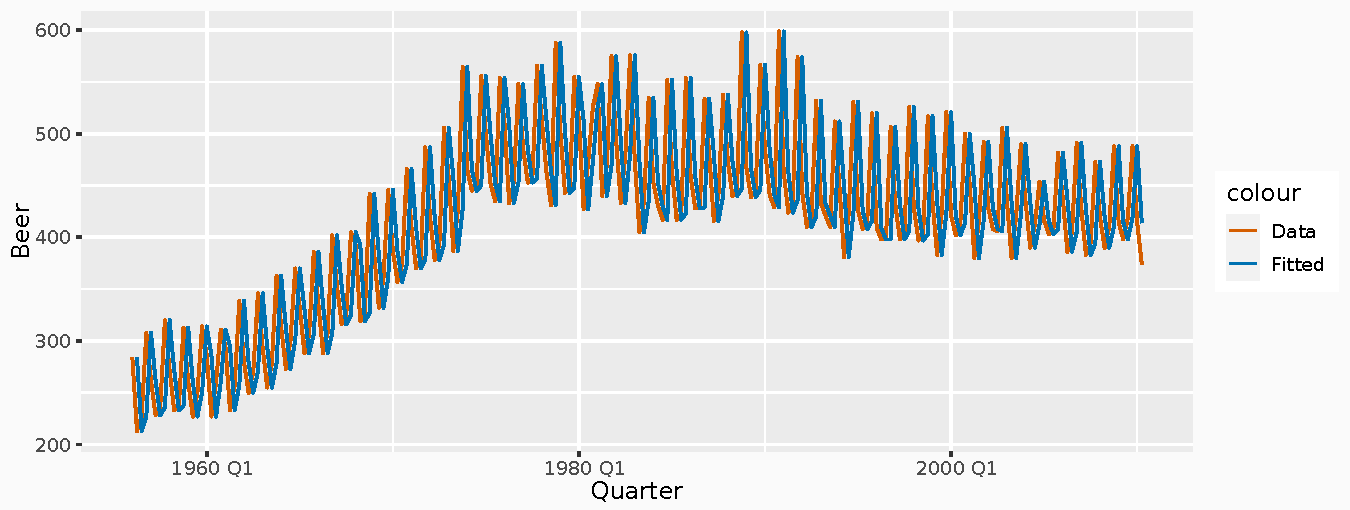
\includegraphics{03_basic_modelling_files/figure-beamer/dj4-1.pdf}
\end{frame}

\begin{frame}[fragile]{Beer production - residuals}
\protect\hypertarget{beer-production---residuals}{}
\fontsize{10}{10}\sf

\begin{Shaded}
\begin{Highlighting}[]
\FunctionTok{augment}\NormalTok{(fit) }\SpecialCharTok{|\textgreater{}}
  \FunctionTok{autoplot}\NormalTok{(.resid) }\SpecialCharTok{+}
  \FunctionTok{labs}\NormalTok{(}\AttributeTok{x =} \StringTok{"Quarter"}\NormalTok{, }\AttributeTok{y =} \StringTok{""}\NormalTok{, }\AttributeTok{title =} \StringTok{"Residuals from naïve method"}\NormalTok{)}
\end{Highlighting}
\end{Shaded}

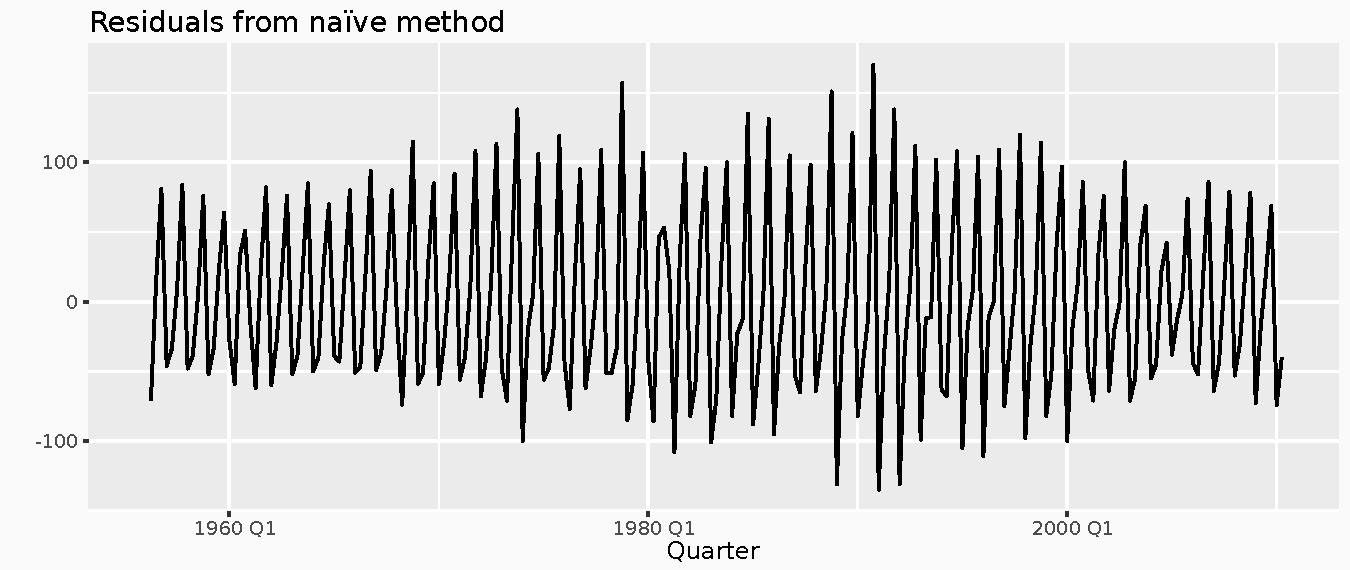
\includegraphics{03_basic_modelling_files/figure-beamer/dj5-1.pdf}
\end{frame}



\end{document}
